\chapter{Analisis}
\label{chap:analisis}

\section{Analisis Sistem Masa Kini}
    
    Analisis sistem yang digunakan pada saat ini di lab komputasi akan dimulai
    dengan menganalisis alur pelaksanaan ujian terlebih dahulu. Kemudian
    dilanjutkan dengan melakukan penyebaran kuisioner untuk mendapatkan
    informasi lebih lanjut tentang masalah yang tidak teridentifikasi pada saat
    survei pelaksanaan ujian.
    
    Kedua sumber informasi tersebut kemudian akan dianalisis untuk membuat
    usulan fitur baru yang akan diimplementasi pada sistem yang baru.

% \subsection{Pelaksanaan Ujian}

    \begin{figure}[H]
        \centering
        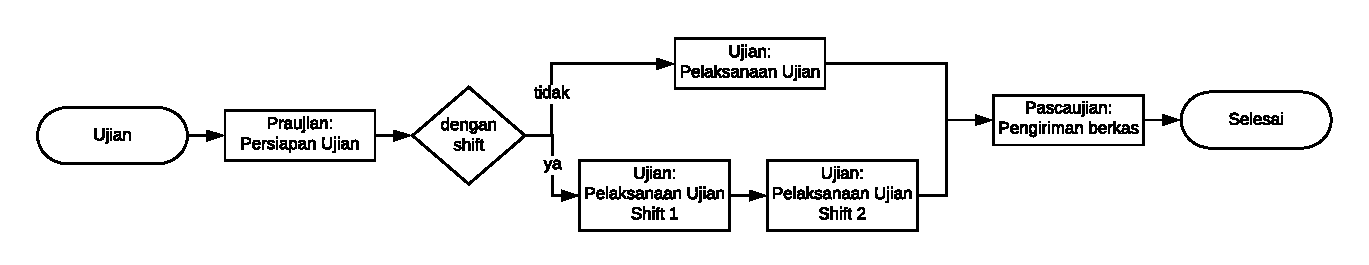
\includegraphics[width=0.75\paperwidth]{Gambar/flowchart/exam-flow-ujian.pdf}
        \caption{Diagram alur pelaksanaan ujian secara garis besar.}
        \label{fig:flowchart-exam-outline}
    \end{figure}
    
    Pada pelaksanaan ujian, terdapat tiga tahap penting yang
    akan dilalui oleh tiap peran. Pada Gambar \ref{fig:flowchart-exam-outline},
    proses ujian dimulai dengan tahap persiapan ujian. Kemudian pada tahap
    berikutnya terdapat pelaksanaan ujian bergantung pada ada atau tidaknya
    \textit{shift} pada ujian tersebut. Kemudian ditutup dengan pengiriman
    berkas ujian pada tahap pascaujian.
    
    \subsection{Praujian}
    
        \begin{sidewaysfigure}
            \centering
            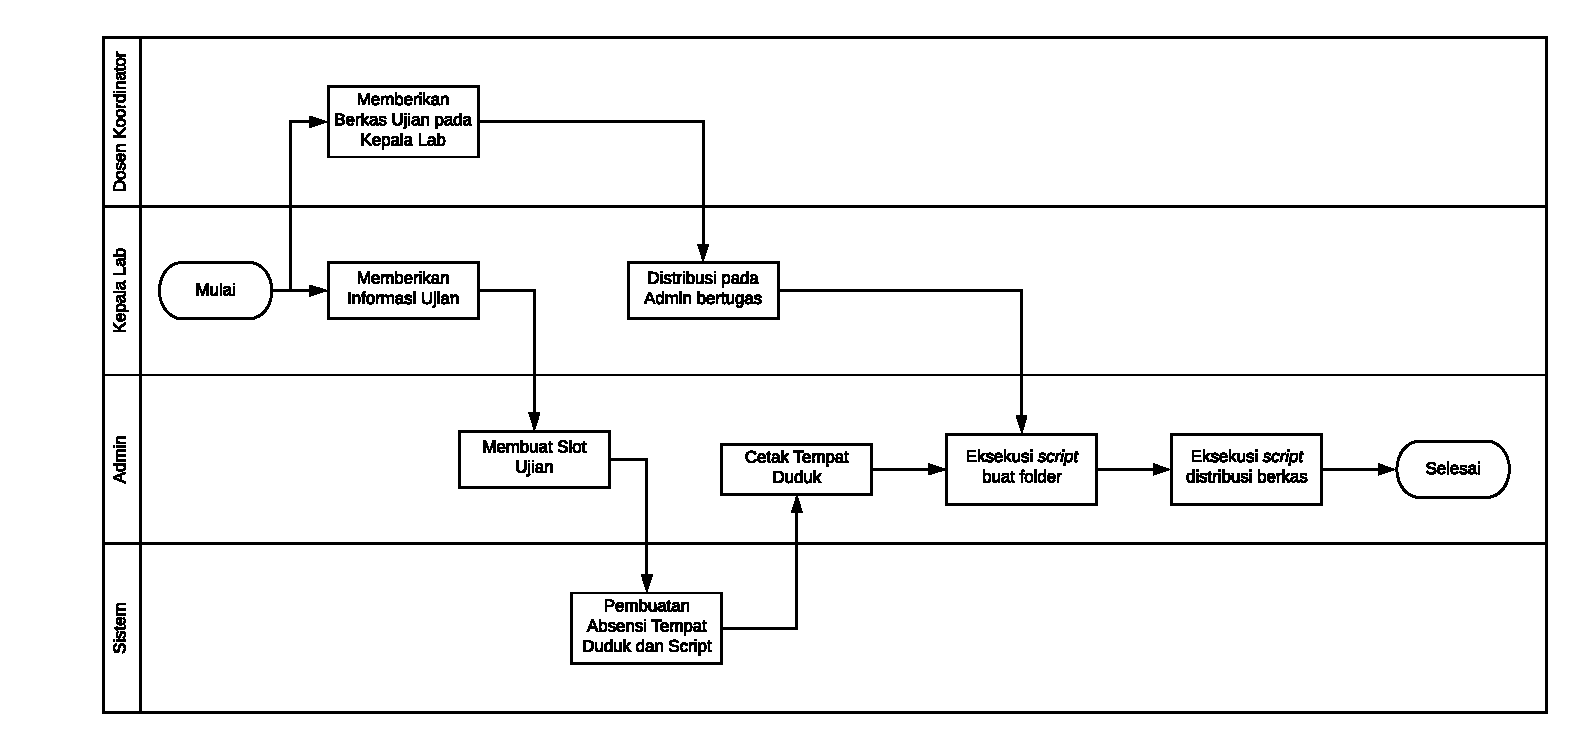
\includegraphics[width=0.75\paperheight]{Gambar/flowchart/exam-flow-ujian-pra.pdf}
            \caption{Diagram alur detil persiapan ujian.}
            \label{fig:flowchart-exam-preexam}
        \end{sidewaysfigure}
        
        Berdasarkan survei lapangan yang dilakukan, persiapan yang dilakukan
        untuk ujian dilakukan beberapa hari sebelum ujian dilaksanakan. Pada
        tahap ini pihak yang terlibat dalam pembuatan slot ujian adalah Admin
        dan Dosen. Alur praujian pada Gambar \ref{fig:flowchart-exam-outline}
        diperjelas pada Gambar \ref{fig:flowchart-exam-preexam} dengan
        mendetilkan masing-masing peran yang terlibat.
        
        Admin akan membuatkan slot ujian pada sistem Oxam, dan mengatur posisi
        tempat duduk sesuai dengan jumlah dan informasi ujian yang diberikan
        dari kepala lab. Sistem kemudian akan menghasilkan daftar tempat duduk
        yang telah diacak oleh sistem. Admin kemudian mencetak daftar tempat
        duduk tersebut untuk nantinya didistribusikan sesuai ruangannya. Dosen
        koordinator yang bertugas untuk membuat soal ujian akan memberikan
        berkas tersebut ke kepala lab. Berkas tersebut kemudian didistribusikan
        pada Admin yang bertugas untuk menjaga ujian.
        
        Sistem juga menghasilkan beberapa \textit{script} dengan fungsi sebagai
        berikut:
        \begin{itemize}
            \item Membuat folder lembar kerja untuk peserta pada masing-masing
                komputer yang telah dimasukkan pada sistem.
            \item Mendistribusikan berkas soal ujian dan berkas bantuan pada
                masing-masing komputer peserta.
            \item Mengambil alih pemilik berkas pada folder lembar kerja peserta
                pada masing-masing komputer.
        \end{itemize}
        
        Persiapan ujian lalu berlanjut pada eksekusi \textit{script} yang
        diberikan oleh aplikasi Oxam. Admin yang bertugas kemudian memasukan
        berkas-berkas ujian pada lokasi khusus di server \textit{deployment}.
        Kemudian script pembuatan folder dan distribusi berkas dieksekusi.
        \textit{Script} yang dieksekusi akan menghasilkan log yang
        menginformasikan keberhasilan pendistribusian berkas tersebut. Admin
        yang bertugas akan memperhatikan log tersebut dan melakukan hal-hal yang
        perlu dilakukan jika terdapat masalah pada log tersebut.
        
        Daftar tempat duduk akan didistribusikan pada pintu lobi dan pintu ruang
        ujian sesaat sebelum ujian dimulai.
    
    \subsection{Ujian}
        \begin{sidewaysfigure}
            \centering
            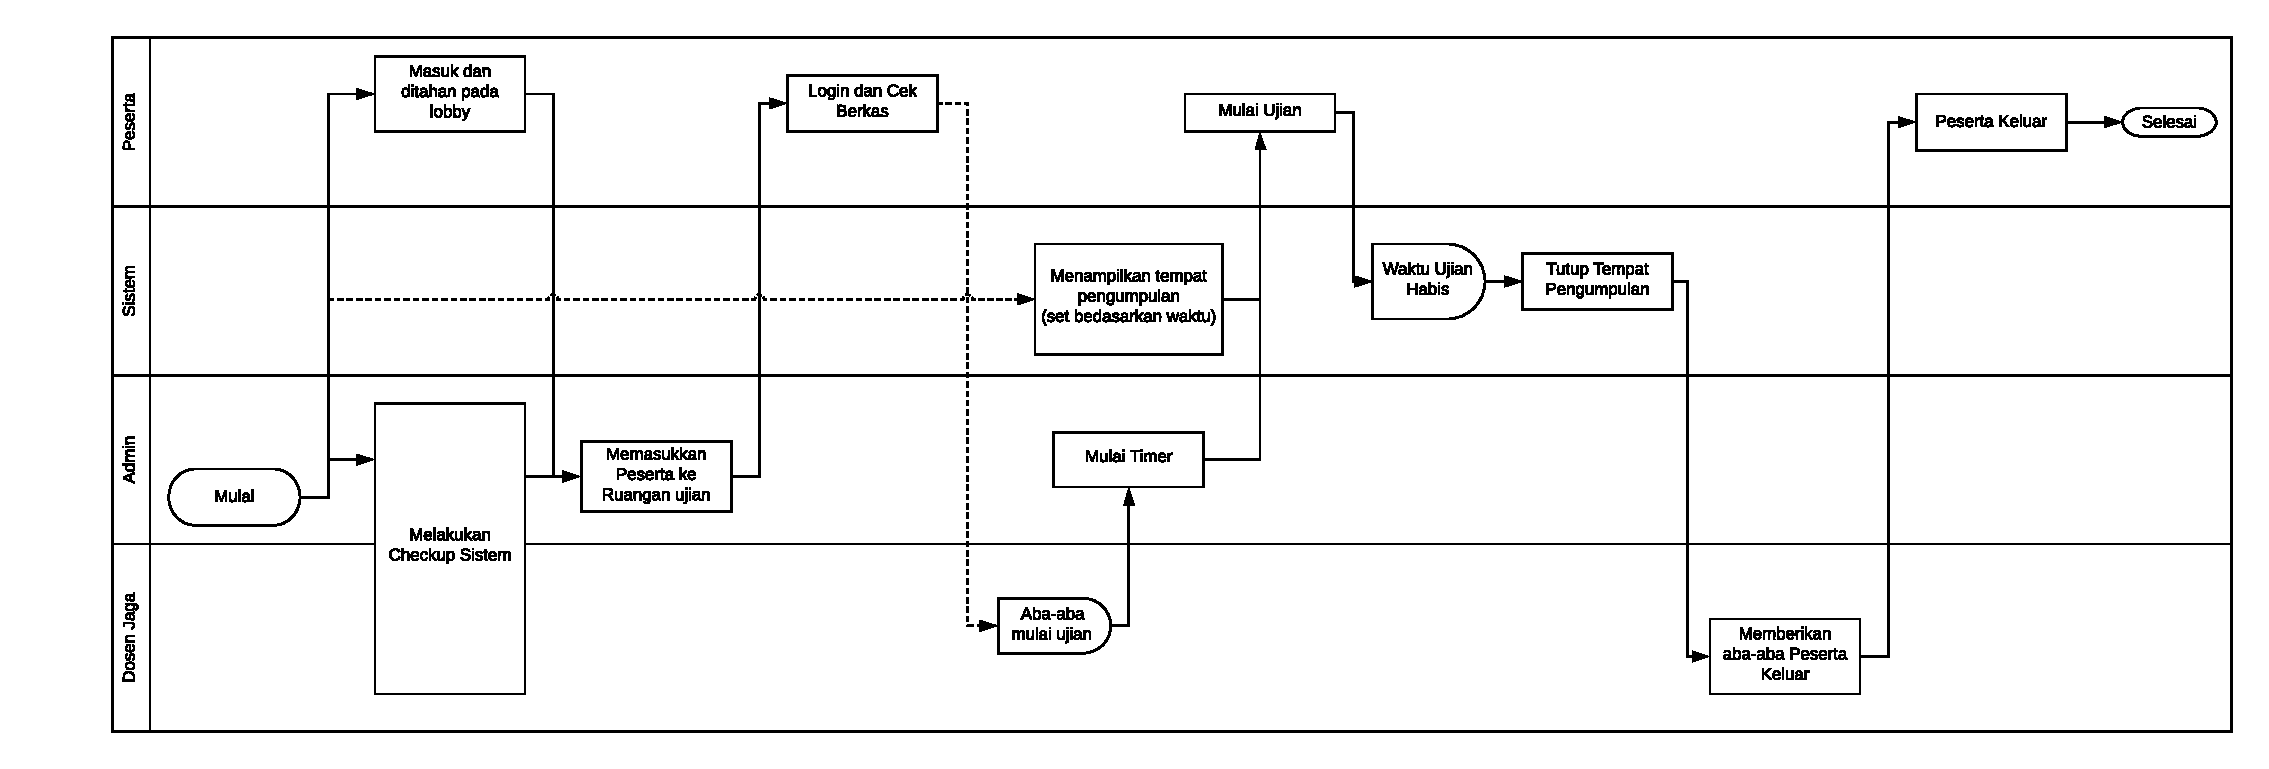
\includegraphics[height=0.8\paperwidth]{Gambar/flowchart/exam-flow-ujian-no-shift.pdf}
            \caption{Diagram alur ujian dengan tanpa \textit{shift}.}
            \label{fig:flowchart-exam-exam-noshift}
        \end{sidewaysfigure}
        % Admin menahan mahasiswa pada lobby
        Proses Ujian kemudian berlanjut pada hari pelaksanaan ujian tersebut
        diadakan. Alur pelaksanaan ujian pada diagram
        \ref{fig:flowchart-exam-outline}, dijelaskan dengan lebih mendetil pada
        diagram \ref{fig:flowchart-exam-exam-noshift}. Peserta yang telah
        diminta hadir 30 menit sebelumnya akan diarahkan untuk masuk dan
        menunggu pada lobi lab. Admin yang bertugas akan memastikan setiap
        peserta yang akan memasuki ruangan ujian telah membawa kartu mahasiswa.
        Dosen ditugaskan untuk menjaga akan melakukan persiapan ujian seperti
        membagikan kertas buram dan sterilisasi ruangan.
        
        % Admin melakukan checkup sekali lagi 
        Sementara itu, Admin beserta dengan dosen yang bertugas untuk menjaga
        selama ujian akan melakukan \textit{check up} terakhir untuk memastikan
        bahwa distribusi soal tidak bermasalah. \textit{Check up} dilakukan
        dengan bantuan daftar check yang telah dibuat Kepala Lab (Lampiran
        \ref{lamp:A}). Pemasangan timer dilakukan pada tahap ini.
        
        % Admin memasukan mahasiswa pada ruang ujian
        Setelah \textit{check up} selesai dan tidak terdapat masalah, admin akan
        membuka sekat pemisah ruang lobi dan ruang ujian. Peserta kemudian masuk
        ke ruangan ujian, dan dipersilahkan duduk sesuai dengan daftar tempat
        duduk yang telah didistribusikan.
        
        % Mahasiswa dipersilahkan login dan melakukan cek berkas bantuan dan
        % ujian (cek ada atau tidak)
        Peserta yang sudah duduk kemudian dipersilahkan untuk segera login dan
        melakukan cek pada berkas ujian tersebut. Peserta yang sudah siap akan
        menunggu aba-aba dari dosen penjaga untuk memulai ujian. Admin yang
        bertugas akan bersiap pada komputer proyektor untuk memulai timer.
        
        % Dosen jaga memberikan aba-aba, Admin start timer & Standby, Mahasiswa
        % mulai ujian
        Pada saat dosen penjaga memberikan aba-aba untuk memulai ujian, admin
        yang bertugas akan memulai timer dan mahasiswa dapat memulai ujian. Slot
        untuk mengumpulkan tempat jawaban akan muncul pada waktu yang
        ditentukan. Peserta ujian dapat melakukan pengunggahan berkas jawaban ke
        portal web dari sistem yang telah dibuka.
        
        % Waktu habis, Dosen jaga beri aba-aba untuk keluar.
        Pada saat waktu ujian telah habis, dosen yang berjaga akan memberikan
        aba-aba untuk peserta menghentikan pengerjaan ujian. Lalu dilanjutkan
        dengan memberikan aba-aba untuk mengeluarkan peserta dari ruangan.
    
    \subsection{Ujian dengan shift}
        \begin{sidewaysfigure}
            \centering
            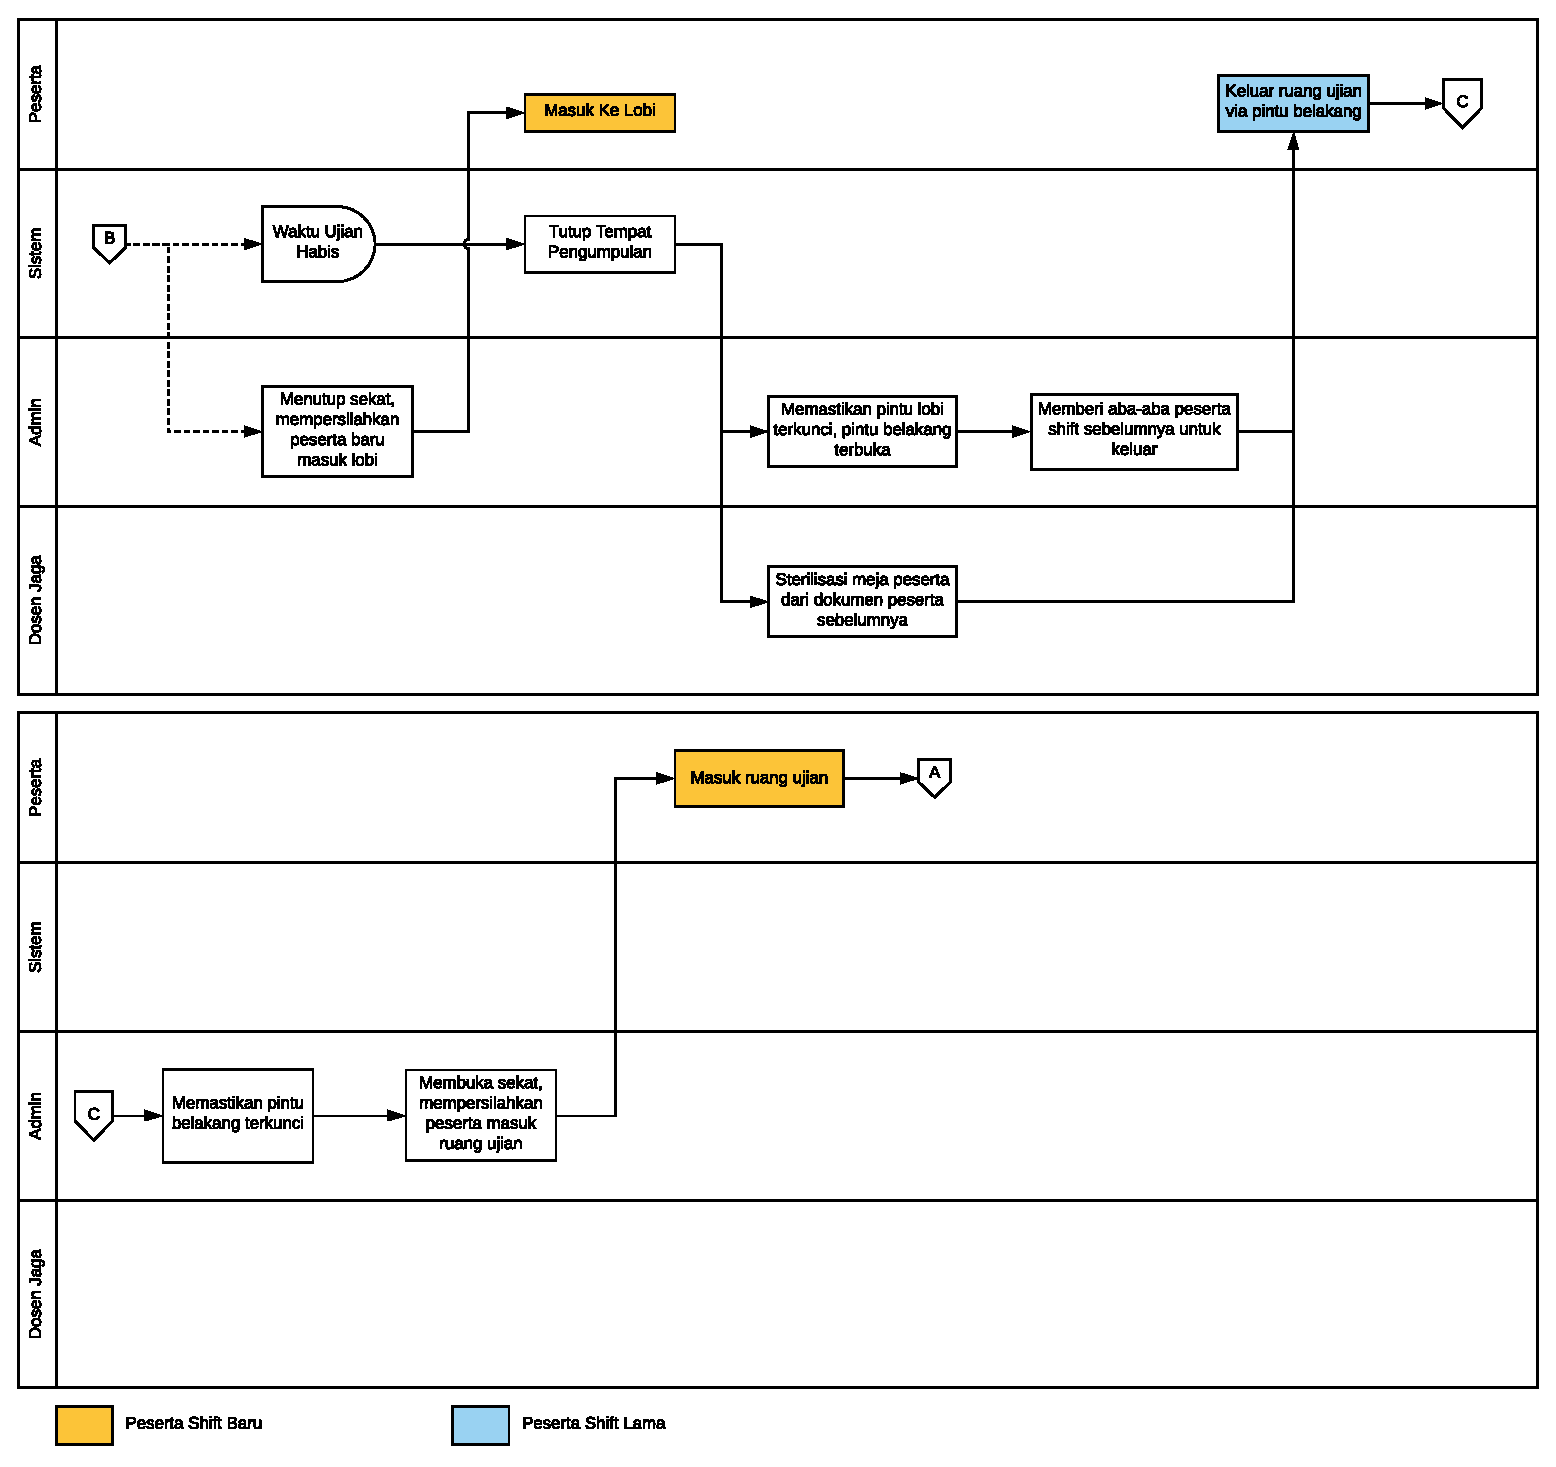
\includegraphics[height=0.8\paperwidth]{Gambar/flowchart/exam-flow-ujian-shift.pdf}
            \caption{Diagram alur ujian dengan shift.}
            \label{fig:flowchart-exam-exam-with-shift}
        \end{sidewaysfigure}
        % Admin memastikan pintu lobby terkunci, sekat menuju ruangan tertutup
        Ujian dengan shift memiliki sedikit perbedaan dalam pelaksanaan ujian.
        Dapat dilihat pada diagram \ref{fig:flowchart-exam-exam-with-shift},
        pebedaan pelaksanaan ini terdapat pada proses memasukan dan mengeluarkan
        peserta antar shift). Pelaksanaan ujian dengan shift ini akan
        mengutamakan isolasi peserta dari peserta yang sudah mengerjakan soal
        ujian. Isolasi tersebut berguna untuk mencegah kecurangan dengan
        membagikan jawaban atau informasi tentang soal pada peserta yang akan
        ujian. Isolasi tersebut dimulai sesaat sebelum waktu ujian pada peserta
        shift sebelumnya telah habis. Admin akan datang pada ruangan untuk
        menahan peserta yang sedang ujian untuk tidak keluar terlebih dahulu.
        Admin lainnya akan memasukan peserta baru ke dalam lobi yang terisolasi.
        Sekat yang memisahkan ruangan lobi dan peserta akan dipasang kembali,
        menahan peserta shift baru tetap di lobi.
        
        % Admin memberikan aba-aba untuk peserta shift sebelumnya keluar lewat
        % pintu belakang
        Saat timer tanda waktu ujian telah habis berbunyi, Admin akan
        berkoordinasi memastikan bahwa pintu lobi telah dikunci dan pintu
        belakang telah dibuka. Admin kemudian akan memberikan aba-aba untuk
        mengeluarkan peserta shift sebelumnya melalui pintu belakang. Dosen yang
        berjaga kemudian melakukan persiapan ujian kembali dengan mensterilkan
        meja peserta dari berkas lama peserta sebelumnya, dan membagikan soal.
        
        % Admin mengunci pintu belakang, Admin membuka sekat menuju ruangan,
        % mempersilahkan peserta masuk
        Setelah peserta ujian pada shift sebelumnya telah keluar sepenuhnya dari
        ruang ujian, Admin akan mengunci pintu belakang, mengisolasi seluruh
        peserta shift baru. Sekat kemudian dibuka dan peserta ujian pada shift
        baru dipersilahkan masuk ke dalam ruangan ujian. Kemudian ujian
        dilakukan sesuai dengan prosedur pelaksanaan ujian seperti biasa.
    
    \subsection{Pascaujian}
        % take own
        Alur ujian berikutnya yang dilalui adalah proses manajemen berkas
        jawaban ujian. Lembar kerja peserta pada komputer yang digunakan
        pertama-tama akan diganti pemilik berkasnya. Berkas yang dimiliki oleh
        peserta ujian tersebut, sekarang menjadi milik akun administrator
        fakultas. Dengan pergantiannya kepemilikan tersebut, akun peserta secara
        efektif tidak akan dapat mengakses, menulis atau pun mengubah berkas
        jawaban tersebut.
        
        % kirim email
        Tim Admin yang bertugas kemudian mengirimkan berkas jawaban yang telah
        diunggah kepada dosen koordinator. Berkas jawaban tersebut pertama-tama
        harus diunduh dari sistem Oxam yang ada secara manual. Kemudian, berkas
        jawaban tersebut dikirim dengan format \textit{archive} seperti zip atau
        rar.

    \subsection{Aplikasi Manajemen Masa Kini}
        Aplikasi yang digunakan untuk ujian masa kini memiliki beberapa fitur
        yang mendukung sistem ujian masa kini. Berdasarkan survei lapangan yang
        dilakukan, aplikasi tersebut memiliki fitur sebagai berikut:
        
        \begin{itemize}
            \item Membuat ujian.
            \item Membuat slot jawaban.
            \item Membuat daftar hadir.
            \item Membuat \textit{script}.
            \item Mengunduh jawaban.
            \item Mengunggah jawaban.
        \end{itemize}

        %% TODO: MORE?

    
\section{Analisis Kebutuhan}
    % Berdasarkan survei dan kuisioner yang dilakukan akan dianalisis poin-poin
    % masalah. Masalah-masalah tersebut akan dikelompokkan berdasarkan peran yang
    % ikut terlibat pada sistem aplikasi ujian.

    Analisis kebutuhan kemudian dilanjut dengan melakukan kuisioner untuk setiap
    peran untuk mengetahui masalah yang terdapat pada tiap pihak. Kemudian dari
    kuisioner tersebut, akan dilakukan analisis untuk mendapatkan poin-poin
    masalah yang ada.

    Kuisioner dibuat secara virtual di Google Forms dan didistribusikan melalui
    sosial media. Kuisioner ini ditujukan pada dua subjek. Subjek pertama adalah
    dosen Koordinator jurusan Informatika yang pernah mengadakan ujian praktik
    di lab. Subjek berikutnya adalah peserta ujian dari jurusan Informatika yang
    pernah mengikuti ujian di lab. 
    
\subsection{Dosen}
    Untuk menganalisis kebutuhan untuk peran dosen, pertama-tama akan dilakukan
    kuisioner terlebih dahulu. Kemudian kuisioner tersebut akan dianalisis untuk
    mendapatkan detil masalah dan solusi yang akan diberikan.

    \subsubsection{Kuisioner}
    Pada subjek dosen, pertanyaan yang diajukan adalah sebagai berikut:
    \begin{itemize}
        \item Apakah Bapak/Ibu puas dengan aplikasi pengumpulan ujian? \\
            Jawaban diberikan dalam bentuk skala 1 (tidak puas) hingga 5 (sangat
            puas). Pertanyaan ini bertujuan untuk mengetahui apakah alur
            pengumpulan ujian sudah nyaman atau belum.
            
        \item Apakah Bapak/Ibu puas dengan format berkas ujian? \\
            Jawaban diberikan dalam bentuk skala 1 (tidak puas) hingga 5 (sangat
            puas). Pertanyaan ini bertujuan untuk mengetahui apakah format
            berkas ujian yang diberikan sudah nyaman digunakan atau belum.
            
        \item Apakah Bapak/Ibu puas dengan pengiriman berkas ujian? \\
            Jawaban diberikan dalam bentuk skala 1 (tidak puas) hingga 5 (sangat
            puas). Pertanyaan ini bertujuan untuk mengetahui apakah alur
            pengiriman berkas ujian via email sudah nyaman atau belum.
            
        \item Apakah Bapak/Ibu puas dengan \textit{judge} ujian (\textit{random
        password}, dsb)? \\
            Jawaban diberikan dalam bentuk skala 1 (tidak puas) hingga 5 (sangat
            puas). Pertanyaan ini bertujuan untuk mengetahui apakah alur
            pemberian informasi kredensial sudah nyaman atau belum.
            
        \item Apakah Bapak/Ibu puas dengan keseluruhan pengalaman berujian di
        lab? \\
            Jawaban diberikan dalam bentuk skala 1 (tidak puas) hingga 5 (sangat
            puas). Pertanyaan ini bertujuan untuk mengetahui apakah alur
            pelaksanaan ujian di lab sudah nyaman atau belum.
            
        \item Masalah apa saja yang biasanya bapak/ibu alami? \\
            Jawaban diberikan dalam bentuk kotak teks yang dapat diisi dengan
            teks yang cukup banyak. Pertanyaan ini bertujuan untuk mengetahui
            masalah yang blum diketahui selama pelaksanaan survei dari sudut
            padang dosen pengawas.
    \end{itemize}

    \begin{figure}
        \centering
        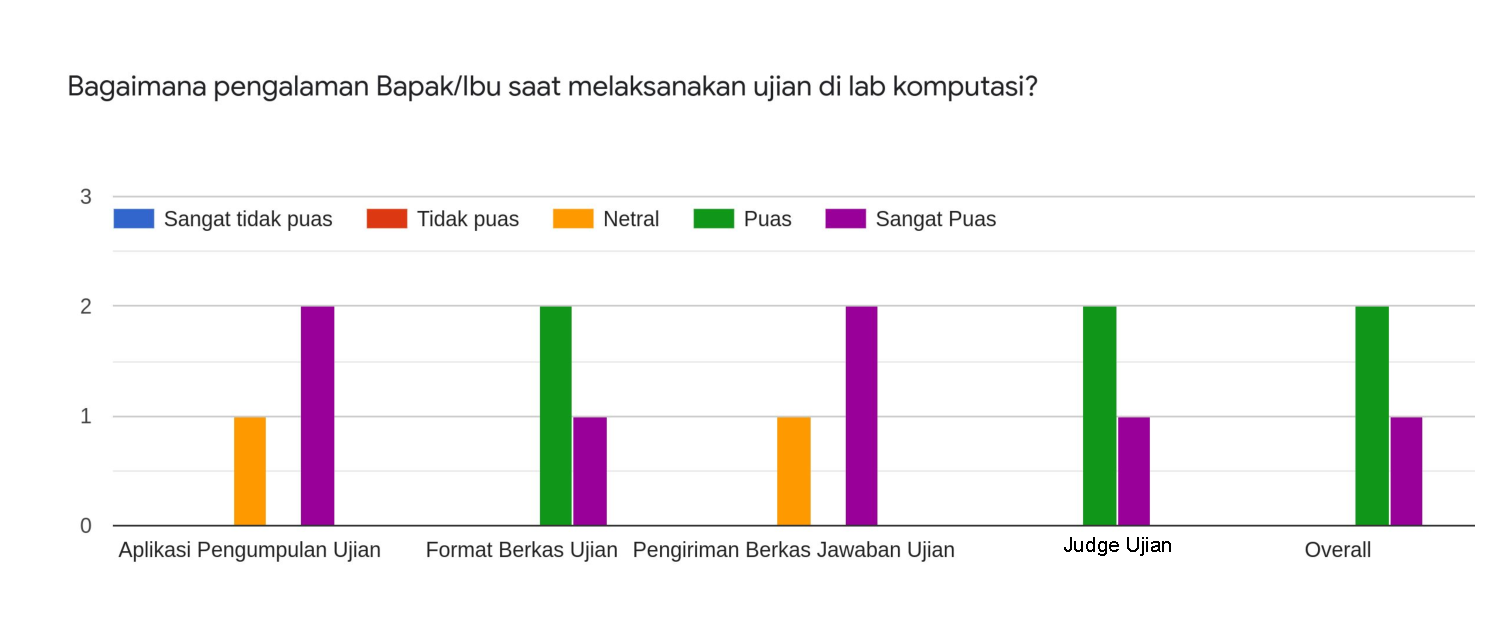
\includegraphics[width=0.6\paperwidth]{Gambar/survey-dosen.pdf}
        \caption{Kuisioner Dosen.}
        \label{fig:kuisioner-dosen}
    \end{figure}

    Pada kuisioner tersebut, terdapat tiga responden yang memberikan respon.
    Tabel grafik dapat dilihat pada gambar \ref{fig:kuisioner-dosen}.
    Berdasarkan respon-respon yang diberikan, dosen-dosen memiliki
    \textit{feedback} yang positif pada sistem ujian yang saat ini telah
    berjalan. Sehingga sistem ujian yang nantinya akan berjalan pada lab dibuat
    memiliki perubahan seminimal mungkin dari sudut padang dosen.

    Pada pertanyaan terakhir, masalah yang dikeluhkan diantaranya:
    \begin{itemize}
        \item Komputer peserta ujian terkadang mengalami \textit{hang}.
        
        \item Hanya ada satu admin yang datang tepat waktu
        
        \item Pertukaran shift kadang membingungkan pengawas, karena pernah
        suatu kali, daftar hadir belum diperbarui
        
        \item Pemberian password kadang masih manual melalui kertas.
        
        \item Kebingungan karena terkadang mahasiswa tidak bisa \textit{submit}
        karena dikatakan "waktu telah habis", tetapi bisa lagi jika
        di-\textit{refresh}.
    \end{itemize}

    Kemudian dari hasil kuisioner tersebut didapatkan beberapa masalah yang
    \subsubsection{\textit{Bug} Waktu Telah
        Habis}\label{ref-prob-dosen-bug-waktu} Laporan masalah pertama berasal
        dari sisi Dosen yang mengawasi ujian di lab komputasi. Masalah yang
        sering kali dikeluhkan adalah \textit{bug} waktu telah habis.
        \textit{Bug} ini didapatkan pada saat peserta sudah membuka halaman
        pengumpulan sudah cukup lama tanpa melakukan penyegaran-ulang
        (\textit{refresh}) ataupun pengumpulan (\textit{submission}). Untuk
        mengatasi masalah ini, biasanya Tim Admin akan meminta peserta ujian
        untuk melakukan penyegaran-ulang beberapa kali hingga pesan kesalahan
        tersebut hilang. Setelah diselidiki, bug tersebut disebabkan oleh
        \textit{cache} yang memiliki umur yang pendek. Umur pendek ini
        menyebabkan \textit{cache} kadaluarsa dan dianggap tidak \textit{valid}
        oleh PHP, sehingga memancing aplikasi untuk memunculkan pesan kesalahan
        tersebut, mencegagh peserta untuk mengumpulkan jawaban pada web.
    
    \subsubsection{Pembagian \textit{Password} yang Masih
        Manual}\label{ref-prob-dosen-password} Masalah berikutnya yang Dosen
        berikan pada kuisioner adalah pembagian \textit{password} yang masih
        manual. Pengujian dengan aplikasi khusus adalah salah satu hal yang
        sering dilakukan di Lab Komputasi. Program tersebut biasanya menggunakan
        otentikasi khusus yang tidak dapat diintegrasikan dengan aplikasi Oxam
        utama untuk mencegah kecurangan. Hal ini saat ini diatasi dengan
        membagikan kertas pada tiap meja, atau membagikannya lewat berkas teks
        pada folder ujian. Sistem ini dilakukan dengan cara melakukan penciptaan
        kata sandi acak yang nantinya dimasukkan pada \textit{script} tertentu.
        Selanjutnya Tim Admin akan melakukan pembuatan akun tersebut dengan
        bantuan \textit{script} tersebut, lalu kredensial tersebut nantinya akan
        diolah untuk nantinya dicetak atau pun dipecah menjadi beberapa berkas
        teks sebelum nantinya diedarkan.

    \subsubsection{Daftar Hadir yang Membingungkan
        Pengawas}\label{ref-prob-dosen-daftar-hadir} Berikutnya, daftar hadir
        yang membingungkan pengawas. Pada hal ini, pengawas kebingungan karena
        kesalahan Tim Admin melakukan pendaftaran peserta. Masalah ini nantinya
        akan didalami pada saat pembahasan survei dari Tim Admin.

\subsection{Peserta}
    \subsubsection{Kuisioner}
    Formulir kuisioner yang dibagikan untuk peserta ujian memiliki pertanyaan
    sebagai berikut:
    \begin{itemize}
        \item Masalah apa saja yang pernah anda alami?\\
            Tujuan pertanyaan ini adalah untuk mengidentifikasi masalah-masalah
            yang sering dialami oleh peserta ujian. Bentuk jawaban adalah daftar
            kotak yang dapat diceklis.
            \begin{itemize}
                \item "Waktu ujian telah habis"
                \item Waktu ujian tidak terlihat dengan baik/jelas
                \item Daftar tempat duduk yang membingungkan
                \item \textit{Credential}\footnote{informasi \textit{login}}
                untuk \textit{Judge} bermasalah
                \item Tidak memiliki masalah
            \end{itemize}
            
        \item Selain dari masalah tersebut, apakah anda memiliki masalah
        lainnya?\\
            Pertanyaan ini ditujukan untuk mengetahui masalah yang tidak
            diketahui oleh Tim Admin atau tidak terlihat secara langsung pada
            saat survei lapangan. Bentuk jawaban adalah kotak teks panjang.
            
        \item Bagaimana pendapat anda tentang ujian di Lab Komputasi?\\
            Pertanyaan ini ditujukan untuk mengetahui pendapat peserta ujian
            tentang pengalaman ujian di lab. Jawaban berupa skala satu hingga
            lima, dengan satu paling buruk, dan lima paling baik.
            
    \end{itemize}
    Kuisioner ditujukan pada peserta ujian yang pernah mengikuti ujian di lab
    pada saat sistem ini masih digunakan. Kuisioner ini direspon oleh 30
    responden yang terdiri dari beberapa angkatan. Berdasarkan respon yang
    diberikan oleh peserta untuk pertanyaan pertama, secara mayoritas masalah
    yang dialami adalah daftar tempat duduk yang membingungkan, diikuti dengan
    masalah \textit{bug} waktu ujian telah habis (Gambar
    \ref{fig:kuisioner-student-1}).
    \begin{figure}
        \centering
        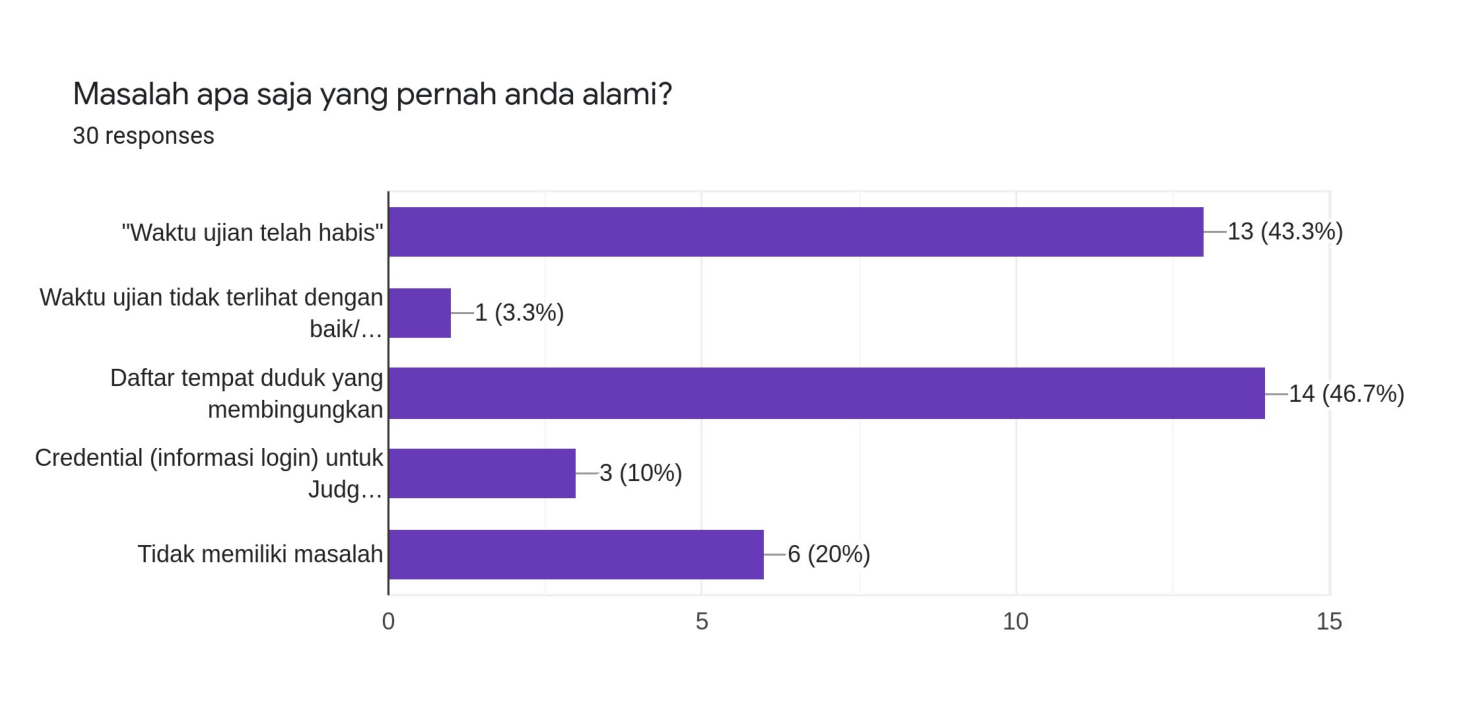
\includegraphics[width=0.7\paperwidth]{Gambar/survey-student.pdf}
        \caption{Respon kuisioner untuk masalah yang telah diketahui pada saat survei.}
        \label{fig:kuisioner-student-1}
    \end{figure}

    Pada pertanyaan kedua, peserta ujian mengeluhkan beberapa masalah seperti:
    \begin{itemize}
        \item Kadang-kadang sesuatu yang ditulis di papan tulis tidak terlihat
        jelas pada posisi duduk tertentu.
        
        \item Beberapa komputer memiliki masalah jaringan
        
        \item Daftar tempat duduk yang miring dan tanpa garis
        
        \item Waktu ujian yang kurang
        
        \item Komputer \textit{hang}
        
        \item Perangkat lunak yang tidak dapat digunakan ketika ujian
    \end{itemize}
    Dari respon-respon tersebut, tidak semua dapat diselesaikan dengan
    mengimplementasikan solusi pada sistem, sehingga masalah-masalah tersebut
    masuk pada batasan masalah.

    Selain itu, secara keseluruhan (lihat Gambar \ref{fig:kuisioner-student-2}),
    peserta ujian memberikan respon yang positif terhadap sistem yang saat ini
    berjalan pada lab. Sehingga pada sisi peserta, perubahan sistem akan dibuat
    seminimal mungkin.

    \begin{figure}
        \centering
        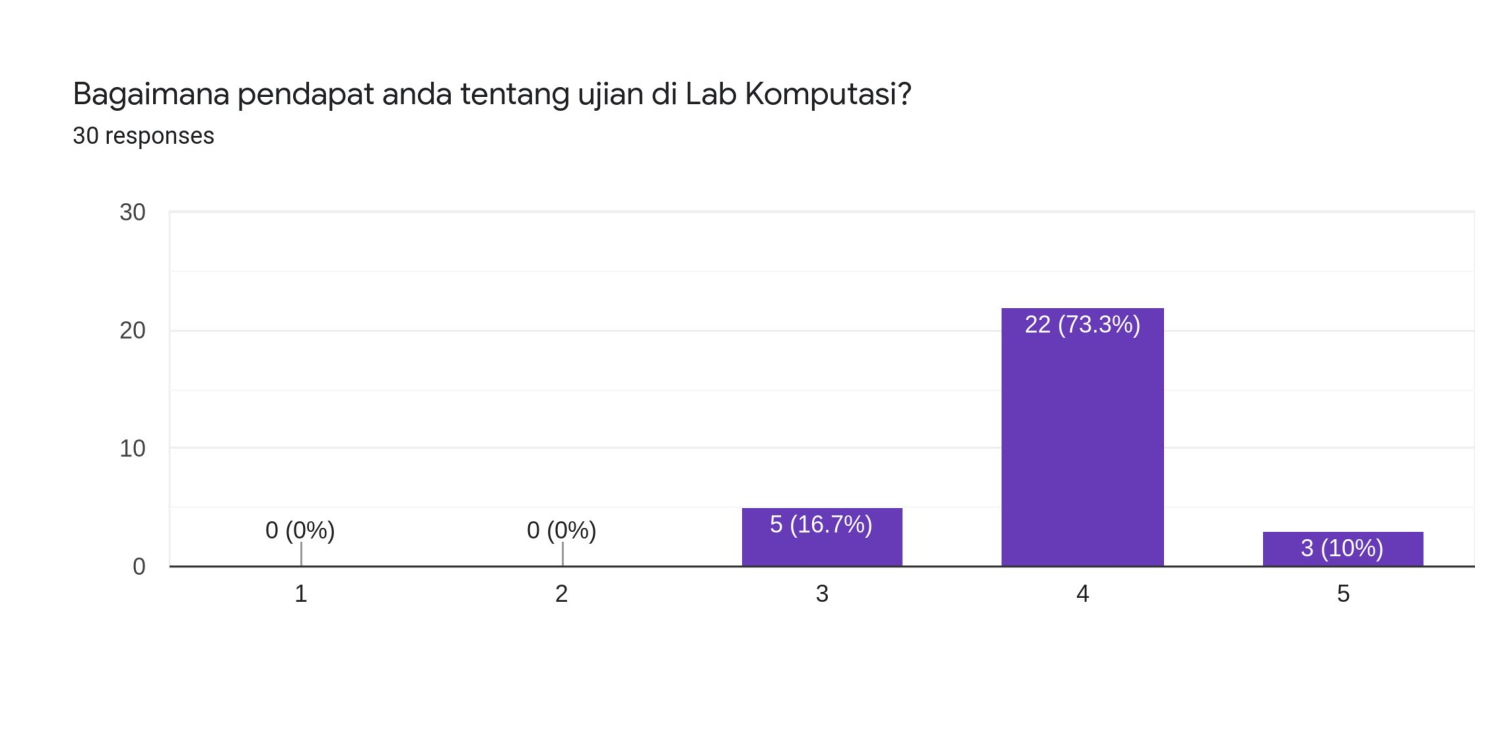
\includegraphics[width=0.7\paperwidth]{Gambar/survey-student-2.pdf}
        \caption{Pendapat peserta ujian pada sistem ujian yang berjalan saat ini.}
        \label{fig:kuisioner-student-2}
    \end{figure}

    \subsubsection{Komputer Hang}\label{ref-prob-peserta-kompu-hang} Kuisioner
    kemudian dilakukan juga untuk peserta ujian yang pernah mengikuti ujian di
    lab komputasi. Dari sisi peserta, Masalah yang muncul pada saat ujian adalah
    komputer yang \textit{hang}. Masalah ini muncul secara acak pada saat ujian
    berlangsung. Peserta biasanya akan diminta untuk direlokasi untuk
    mendapatkan komputer yang tidak bermasalah. Peserta akan diberikan waktu
    tambahan sesuai dengan durasi lamanya komputer tidak dapat digunakan hingga
    komputer peserta yang baru diberikan dapat digunakan kembali. Pada kasus
    ini, masalah tersebut masuk dalam batasan masalah yang tidak dapat diatasi.
    
    \subsubsection{Tulisan Pada Papan Tulis yang Tidak
    Terlihat}\label{ref-prob-peserta-papan-tulis} Selain itu, peserta
    mengeluhkan bahwa tulisan yang ada di papan tulis seringkali tidak terlihat.
    Pada ujian, biasanya informasi seperti kata sandi untuk membuka berkas soal,
    informasi \textit{URL} untuk masuk ke dalam sistem informasi, atau revisi
    soal biasanya ditulis pada papan tulis yang ada di depan. Masalah yang
    timbul adalah peserta yang mendapatkan tempat yang terjauh dari papan tulis
    mengaku kesulitan dalam melihat informasi tersebut. Hal ini dinilai tidak
    adil untuk peserta yang duduk dekat dengan papan tulis, sehingga
    dibutuhkannya fitur untuk memberi tahu informasi ini.

\subsection{Tim Admin}
    \subsubsection{Menghapus Berkas yang
    Gagal}\label{ref-prob-admin-berkas-gagal} 
    Dari sisi Tim Admin, survei yang
    dilakukan menghasilkan banyak keluhan dan masukan. Salah satunya, Tim Admin
    mempermasalahkan bahwa mereka tidak dapat menghapus berkas-berkas yang gagal
    di \textit{deploy}. Masalah tersebut biasanya muncul pada saat Tim Admin
    melakukan kesalahan memasukan data pada saat pembuatan ujian pada aplikasi
    Oxam. Tim Admin yang tidak mengetahui kesalahan tersebut dapat saja
    melakukan \textit{deployment} terlebih dahulu sebelum akhirnya menyadari
    bahwa ia telah melakukan kesalahan. Masalah yang dikeluhkan berakar dari
    fodler yang tidak digunakan tersebut membingungkan bagi peserta dan
    berpotensi menjadi celah keamanan untuk mencontek.

    Selain folder, Tim Administrator juga harus menghapus daftar yang ada pada
    database. Setelah diselidiki, masalah timbul dari \textit{record} yang
    ditandai sebagai di hapus dengan mengisi kolom \texttt{isDeleted} menjadi
    \texttt{1}, namun tidak membuat sistem pengumpulan berubah. Masalah yang
    timbul adalah sebagian dari peserta mendapatkan tempat pengumpulan yang
    berbeda dari seharusnya.

    \subsubsection{Pindah Tempat Duduk Peserta}\label{ref-prob-admin-pindah}
    Selain itu, beberapa masalah lainnya adalah pindah tempat duduk peserta.
    Bersinggungan dengan masalah yang dimiliki peserta tentang komputer yang
    \textit{hang} pada \ref{ref-prob-peserta-kompu-hang}, Tim Administator
    memiliki kesulitan untuk melakukan pemindahan komputer karena Aplikasi yang
    saat ini ada memiliki masalah tentang mengubah posisi tempat duduk. Masalah
    yang muncul adalah dibutuhkannya orang untuk melakukan:
    \begin{itemize}
        \item Pemindahan peserta
        \item Pemindahan berkas ujian peserta
        \item Pemindahan \textit{record} pada database Oxam
    \end{itemize}

    Dengan begitu jika terdapat lebih dari seorang peserta yang mengalami
    masalah ini maka dibutuhkan waktu yang sangat lama untuk menyelesaikan
    masalah tersebut.

    \subsubsection{Pengiriman Berkas Jawaban
    Otomatis}\label{ref-prob-admin-pengiriman-berkas} 
    Normalnya, setelah ujian
    selesai maka Tim Admin akan mengunduh berkas jawaban tersebut untuk
    dikirimkan ke Dosen Koordinator. Tim Admin akan mengakses aplikasi Oxam,
    lalu mengunduh berkas jawaban ujian dan mengirimnya secara manual ke Dosen
    Koordinator mata kuliah tersebut. Masalah yang muncul adalah tidak setiap
    kali ujian Tim Admin ingat untuk mengirimkan berkas.
    
    \subsubsection{NPM Jenis Baru}\label{ref-prob-admin-npm-baru} 
    Peserta yang
    menjalani ujian praktik pada lab komputasi adalah mahasiswa. Bergantinya
    sistem informasi akademik kampus berdampak pada pergantian format NPM yang
    dimiliki oleh mahasiswa. NPM pada mahasiswa memiliki format tertentu yang
    dapat menginformasikan asal dari mahasiswa tersebut.

    \begin{table}[H]
        \centering
        \def\arraystretch{2}
        \begin{tabular}{|c|c|}
            \hline
            \textbf{NPM Lama} & \textbf{NPM Baru} \\
            \hline
            201673\textbf{0011} & 6181601\textbf{011} \\
            \hline
            \multicolumn{2}{|c|}{\textbf{username}} \\
            \hline
            \multicolumn{2}{|c|}{i16\textbf{011}} \\
            \hline
        \end{tabular}
        \caption{NPM lama, baru dan username yang mahasiswa gunakan untuk login.}
        \label{tab:table-npm-detail}
    \end{table}
    
    NPM lama memiliki empat komponen besar yang digunakan untuk mengidentifikasi
    jenis mahasiswa (Tabel \ref{tab:table-npm}, kolom NPM Lama). 
    \begin{itemize}
        \item Empat karakter pertama pada NPM adalah informasi tahun mahasiswa
        tersebut memulai kuliah. Pada contoh tampak angka 2016, yang berarti
        mahasiswa tersebut memulai perkuliahannya pada tahun 2016 (angkatan 2016). 
        
        \item Dua karakter berikutnya menandakan jurusan (dan fakultas) mahasiswa
        tersebut belajar. Pada contoh tampak angka 73 yang menandakan bahwa
        mahasiswa tersebut belajar pada Fakultas Teknologi Informasi dan Sains (7),
        dan berada pada jurusan Informatika (73). 
        
        \item Satu karakter berikutnya menandakan program yang diambil oleh
        mahasiswa tersebut. Angka 0 menunjukkan bahwa mahasiswa tersebut mengikuti
        program Sarjana, seperti pada tabel contoh. Angka 1 menandakan mahasiswa
        tersebut mengambil program pascasarjana dan angka 2 menunjukkan program
        doktoral. 
        
        \item Tiga angka berikutnya yang menjadi komponen terakhir dari NPM lama ini
        adalah nomor urut mahasiswa tersebut. Dengan spesifikasi berikut,
        berdasarkan tabel contoh, mahasiswa dengan NPM 2016730011 adalah mahasiswa
        angkatan 2016, mengikuti program sarjana informatika pada Fakultas Teknologi
        Informasi dan Sains dengan nomor urut 11.
    \end{itemize}
    
    NPM baru ini dibuat pada tahun 2018, dan memiliki struktur yang jauh berbeda
    dari NPM lama. Format NPM tersebut didefinisikan sebagai berikut:
    
    \begin{itemize}
        \item Angka pertama menandakan program jenjang yang diambil oleh mahasiswa
        tersebut. Angka 5 untuk diploma, 6 untuk sarjana, 8 pascasarjana dan 9 untuk
        doktoral. 
    
        \item Dua digit angka berikutnya menunjukkan program studi yang diambil oleh
        mahasiswa tersebut, pada contoh 18 berarti Informatika. 
        
        \item Dua digit berikutnya menunjukan angka tahun mulai perkuliahan
        (angkatan) dalam format representasi tahun dengan dua digit. Pada contoh
        tampak angka 16 yang berarti mahasiswa tersebut adalah angkatan 2016. 
        
        \item Dua digit berikutnya menginformasikan jenis mahasiswa. Pada contoh
        tampak angka 01 yang menandakan bahwa mahasiswa tersebut berjenis reguler.
        
        \item Tiga digit terakhir menginformasikan nomor urut mahasiswa tersebut.
    \end{itemize}
    
    Pada tabel \ref{tab:table-npm-detail} terdapat kolom username yang digunakan
    untuk menstandarisasi NPM tersebut. Informasi username ini nantinya
    dimanfaatkan untuk mengintegrasi berbagai macam sistem yang membutuhkan
    informasi mahasiswa. Digit pertama pada username menginformasikan jurusan
    mahasiswa tersebut. Huruf \texttt{i} menginformasikan mahasiswa tersebut
    adalah mahasiswa jurusan Informatika, huruf \texttt{m} untuk matematika, dan
    huruf \texttt{f} untuk fisika. Dua digit berikutnya menginformasikan tahun
    angkatan mahasiswa tersebut dalam bentuk representasi tahun dalam dua digit.
    Pada contoh tampak angka 16, yang menandakan bahwa username ini adalah milik
    mahasiswa angkatam 2016. Tiga digit terakhir berikutnya menginformasikan
    nomor urut mahasiswa tersebut.
    
    \subsubsection{Kode Matakuliah Baru}\label{ref-prob-admin-kode-mk-baru}
    Kurikulum yang saat ini ada memikili kode matakuliah yang baru. Masalah yang
    muncul adalah sistem aplikasi yang lama tidak memiliki admin panel untuk
    melakukan manajemen mata kuliah yang baru.
    
    \subsubsection{Timer yang tidak
    terintegrasi}\label{ref-prob-admin-timer-integrated} Pada saat pelaksanaan
    ujian, Tim Admin menggunakan timer yang disediakan oleh sistem operasi
    Windows. Masalah yang timbul adalah buka dan tutupnya tempat pengumpulan
    ujian tidak berjalan bersamaan dengan timer. Sebagai contoh, pada saat timer
    menunjukan waktu sudah habis, peserta masih dapat mengumpulkan berkas ujian.
    
    
\subsection{Analisis Fitur Aplikasi}
    Berdasarkan survei yang dilakukan dan kuisioner yang disebar, didapatkan
    beberapa masalah yang menandakan bahwa aplikasi pendukung ujian di lab
    komputasi belum efektif membantu pelaksanaan ujian. Masalah-masalah tersebut
    akan diselesaikan dengan merekayasa ulang aplikasi yang telah ada pada
    sistem yang lama. Rekayasa ulang tersebut dilakukan dengan bantuan
    \textit{framework} agar sumber kode yang dibuat dapat dirawat oleh tim
    Admin.
    
    \subsection{Timer Tidak Terintegrasi}
        Sesuai dengan kebutuhan yang dijelaskan pada
        \ref{ref-prob-admin-timer-integrated}, timer akan diimplementasi secara
        terintegrasi. Timer nantinya akan menutup tempat jawaban pada saat waktu
        telah habis. Timer harus dapat mengatur buka tutupnya tempat pengumpulan
        jawaban peserta.
    
    \subsection{Notifikasi}
        Fitur pertama yang ingin ditambahkan adalah sistem notifikasi. Fitur ini
        nantinya akan menyelesaikan masalah pada keluhan kata sandi yang
        disebarkan manual (\ref{ref-prob-dosen-password}), dan informasi yang
        dituliskan di papantulis tidak terlihat
        (\ref{ref-prob-peserta-papan-tulis}). Dosen pengawas nantinya dapat
        membuat buah notifikasi baru untuk peserta dan peserta dapat langsung
        melihat notifikasi tersebut pada tempat pengumpulan.

    \subsection{Pemindahan Tempat Duduk Peserta}
        Fitur kedua yang ingin ditambahkan adalah fitur pemindahan tempat duduk
        peserta. Fitur ini nantinya akan
        menyelesaikan masalah peserta yang mengalami \textit{hang} pada saat
        ujian berlangsung (\ref{ref-prob-peserta-kompu-hang}) dan Tim Admin yang
        ingin memindahkan tempat duduk peserta(\ref{ref-prob-admin-pindah}). Fitur ini nantinya hanya
        akan dapat digunakan oleh Tim Admin. Dosen pengawas diharapkan untuk
        mengkontak Tim Admin untuk melakukan perpindahan untuk memastikan
        komputer yang baru akan memiliki kemungkinan bermasalah yang lebih
        kecil.

    \subsection{Pengiriman berkas otomatis}
        Fitur lainnya adalah perngiriman berkas otomatis. Fitur ini untuk
        menyelesaikan masalah pada pengiriman berkas jawaban ujian oleh Tim
        Admin (\ref{ref-prob-admin-pengiriman-berkas}). Pada dasarnya fitur ini
        dapat implementasi dengan cara membuat \textit{cronjob} setiap menit
        yang nantinya mengecek apakah terdapat berkas ujian yang dapat di kirim.
        Pengiriman dapat berlangsung secara otomatis lewat email.

    \subsection{NPM \textit{Converter}} NPM \textit{Converter} nantinya akan
        mengabstraksi seluruh NPM yang saat ini aktif di sistem UNPAR. Abstraksi
        tersebut nantinya diharapkan dapat menstandarisasi dua format yang saat
        ini berjalan.
        
    \subsection{Admin Panel}
        Admin panel ditambahkan dengan tujuan agar dapat memanajemen seluruh
        entitas database pendukung ujian. Sebagai contoh, penambahan atau
        penghapusan mata kuliah. Saat ini, pada sistem yang aktif tidak terdapat
        tempat untuk menambahkan atau menghapus mata kuliah.
    
    \subsection{Bug \textit{fix}} Implementasi sisanya, terdapat beberapa
        masukan yang dapat dilakukan, yaitu untuk menyelesaikan masalah tentang
        \textit{bug} waktu ujian telah habis (\ref{ref-prob-dosen-bug-waktu})
        dapat diimplementasi dengan melakukan authentikasi berdasarkan IP yang
        tidak disimpan menggunakan \textit{cache} atau \textit{session}. Hal ini
        memperkecil masalah \textit{cache} atau \textit{session} yang kadaluarsa
        karena waktu yang diberikan terlalu kecil. Sehingga setiap kali koneksi
        dijalankan dari klien ke \textit{server}, server akan langsung mengecek
        IP tersebut dengan yang ada di database melakukan apapun.

\section{Analisis Pemilihan Framework dan Library}
%- Pake framework biar daapt di extend oleh penerus
Penggunaan \textit{framework} diharapkan dapat membuat aplikasi dikembangkan
lebih lanjut oleh penerus Tim Admin berikutnya. Sifat \textit{framework} yang
dapat digunakan-ulang dan modular membuat \textit{framework} memiliki pola yang
dapat dipelajari dengan cepat. Memungkinkan Tim Admin untuk dapat menambahkan
fitur baru dengan lebih cepat. 

Berdasarkan survei yang dilakukan oleh StackOverflow pada tahun
2018\cite{stackoverflow:survey-2018} dan 2019\cite{stackoverflow:survey-2019},
PHP adalah salah satu bahasa yang mayoritas digunakan oleh pengembang aplikasi
web. Dengan banyaknya pengguna bahasa tersebut, maka komunitas, \textit{library}
dan firum akan lebih besar. Pilihan tersebut dinilai lebih menguntungkan karena
pengembang hanya perlu mempelajari cara menggunakan \textit{library} tersebut
tanpa harus mengimplementasi algoritmanya dari dasar. Dengan begitu banyaknya
pilihan yang ada, developer yang ingin menambahkan fitur tersebut dapat lebih
berfokus untuk mengimplementasi fitur tersebut.

\subsection{FatFree Framework}

\begin{figure}[H]
    \centering
    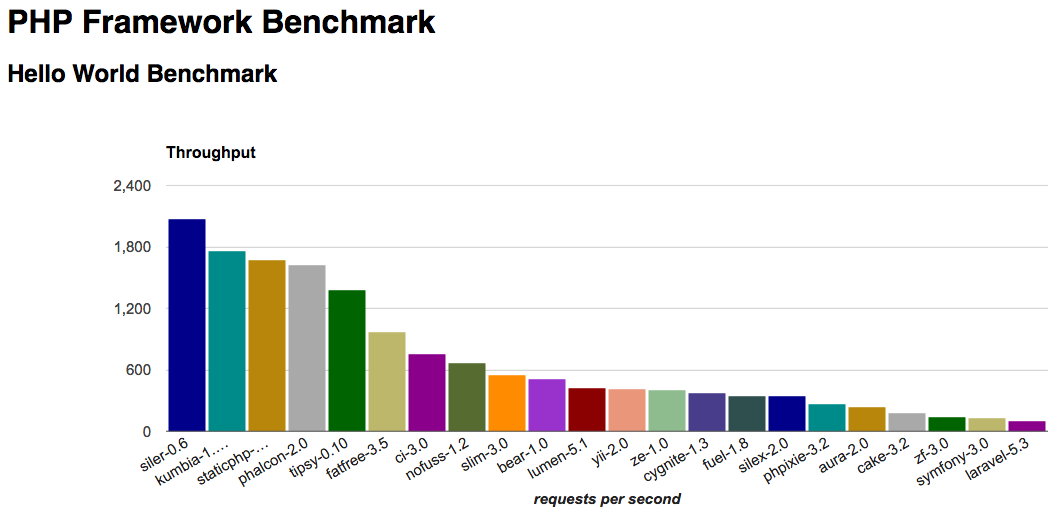
\includegraphics[width=0.6\paperwidth]{Gambar/php-framework-benchmark-20170214.png}
    \caption{Hasil \textit{benchmark} terhadap beberapa \textit{framework} pada
        bahasa pemrograman PHP\protect\cite{kenjis:framework-benchmark}. (Lebih
        tinggi lebih baik)}
    \label{fig:chart-benchmark-php-framework}
\end{figure}

%- Karena penggunaan fleksibel
Beberapa \textit{framework} memiliki sifat yang fleksibel, sehingga memungkinkan
developer mengadopsi \textit{framework} tersebut dengan gaya mereka masing-masing.
Fat-Free \textit{framework} tidak memiliki pola pemrograman yang pasti, namun sistem
mereka dirancang agar dapat digunakan pada tipe pola pemrograman apapun. Kontras
dengan \textit{framework} besar seperti Laravel, atau Code Igniter. Fat-free sendiri
dengan jelas menuliskan untuk menggunakan gaya apapun yang pengembang
butuhkan\footnote{https://fatfreeframework.com/3.6/getting-started\#EnoughSaid-SeeForYourself}.
 
Dengan sifat analisis kebutuhan yang cepat, maka penggunaan \textit{framework} yang kecil
dan ringan dibutuhkan. Selain itu dengan kebutuhan yang mengharuskan
implementasi cukup fleksibel untuk kemudian hari dikembangkan lebih lanjut, maka
FatFree Framework atau F3 akan digunakan untuk penelitan ini.

\subsection{React.js}
    Menurut survey yang dilakukan oleh StackOverflow pada tahun 2019, Reactjs
    adalah salah satu \textit{framework} javascript yang paling banyak digunakan
    pada
    web\footnote{https://insights.stackoverflow.com/survey/2019{\#}technology-{\_}-web-frameworks}.
    Selain itu menurut survey tersebut, Reactjs adalah salah satu \textit{framework} yang
    paling disukai oleh pengembang. Dengan dua alasan tersebut penelitian ini
    menggunakan Reactjs sebagai \textit{framework} Frontend.

\subsection{CI/CD}
    Penggunaan \textit{library} React pada front-end membutuhkan tahap tambahan
    untuk melakukan \textit{build} sebelum subsistem dapat dijalankan di
    peramban pengguna. Adanya tahap tambahan ini membuat penelitian ini
    membutuhkan sebuah sistem \textit{build} terpusat untuk mempermudah
    mengelola kode sumber yang akan di-\textit{deploy} pada server produksi.
    Sistem build ini akan diimplementasi dengan menggunakan teknologi CI/CD yang
    disediakan oleh penyedia penyimpanan kode sumber, GitLab.
    
    Sistem CI/CD nantinya harus dapat berjalan hampir otomatis seluruhnya untuk
    menyederhanakan alur pengembangan aplikasi. Sistem CI/CD ini diharapkan
    untuk mempermudah pekerjaan pengembang untuk melakukan \textit{build} dengan
    standar produksi dengan package dan modules untuk development tidak
    diikutkan pada hasil \textit{build}. Harapan lainnya adalah dengan adanya
    CI/CD ini, pengembang dapat menambahkan \textit{routine} apapun yang
    dibutuhkan dikemudian hari.

\section{Analisis Pengguna}
\begin{figure}[thb]
    \centering
    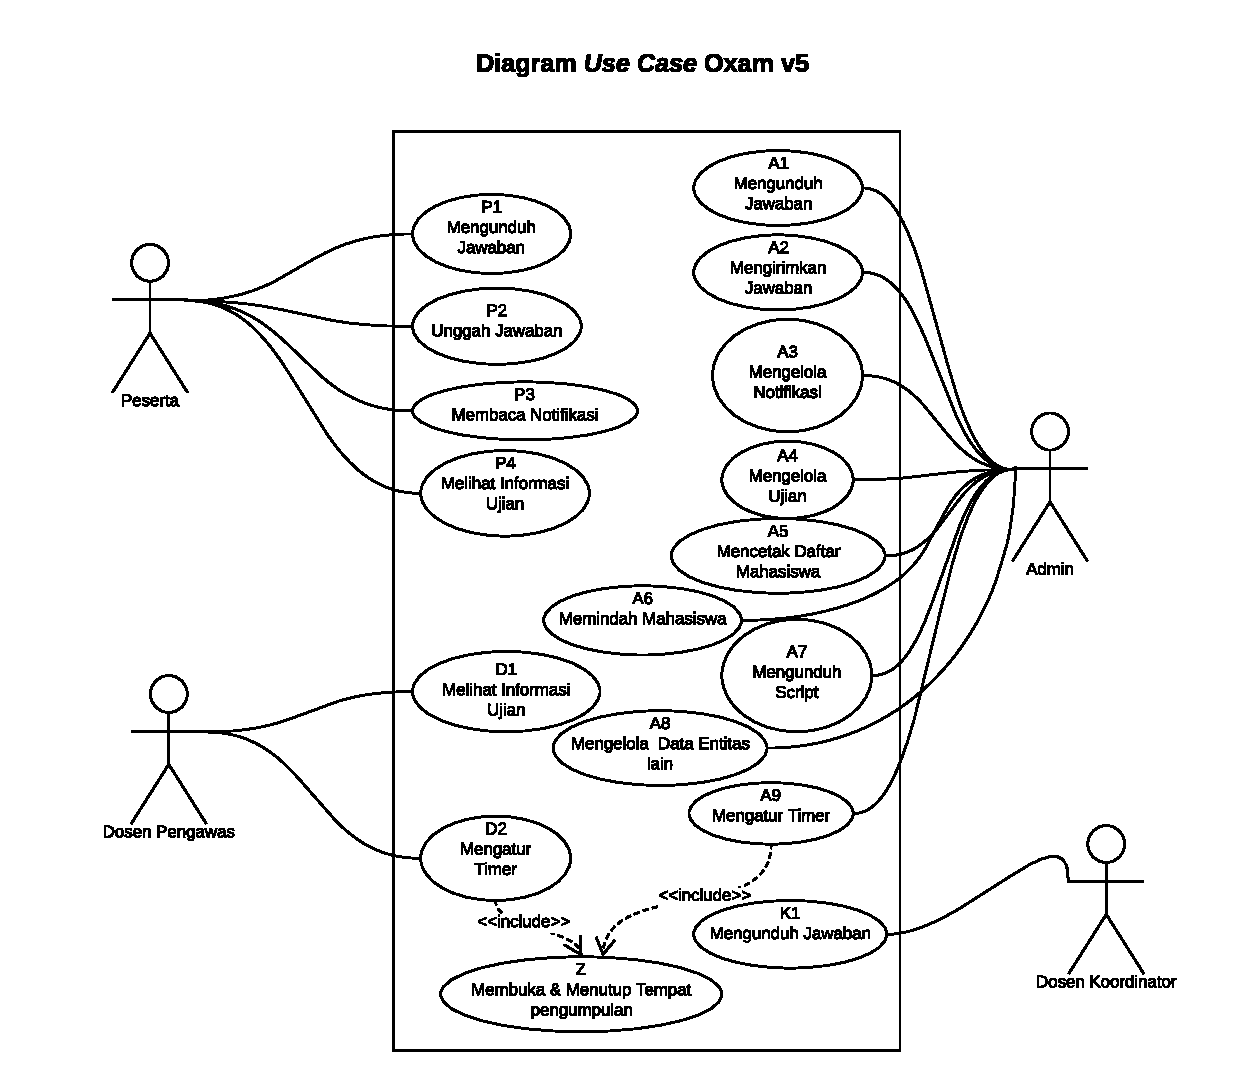
\includegraphics[width=0.6\paperwidth]{Gambar/UseCase - RevB.pdf}
    \caption{Diagram \textit{Use Case} untuk aplikasi Oxam yang baru.}
    \label{fig:diagram_usecase}
\end{figure}

Pengguna aplikasi sistem Oxam yang ada saat ini terdapat tiga pihak utama.
Pihak pertama adalah Tim Admin yang bertugas untuk menyiapkan ruangan
untuk ujian. Pihak kedua adalah peserta. Peserta adalah subjek yang akan
menggunakan ruangan ujian. Pihak ketiga adalah dosen. Dosen terdiri dari
dua tugas, dosen pengawas, dan dosen koordinator. Dosen pengawas akan melakukan
pengawasan terhadap pelaksanaan ujian, sedangkan dosen koordinator adalah
dosen yang akan memberikan ujian, dan mengkoodinasikan dosen pengawas.

Diagram \textit{use case} dari aplikasi ini dapat dilihat pada Gambar 
\ref{fig:diagram_usecase}. Pada diagram terdapat empat kasus penggunaan berdasarkan
perannya. Untuk peran dosen, peran dibagi menjadi dua berdasarkan tugasnya. 
Informasi lengkap tentang penggunaan tiap peran dapat dilihat pada Tabel \ref{tab:usecase_desc}.

\begin{table}[ht]
    \centering
    \begin{tabularx}{\textwidth}{|p{1.2cm}|p{2cm}|X|}
         \hline
         Nomor & Peran & Deskripsi  \\
         \hline
         P1 & Peserta & Peserta dapat mengunduh berkas jawaban yang telah mereka unggah. \\
         \hline
         P2 & Peserta & Peserta dapat mengunggah berkas jawaban pada slot jawaban yang tersedia. \\
         \hline
         P3 & Peserta & Peserta dapat membaca notifikasi yang diberikan oleh sistem. \\
         \hline
         P4 & Peserta & Peserta dapat melihat informasi ujian. \\
         \hline
         A1 & Admin & Tim Admin akan dapat mengunduh seluruh jawaban yang telah peserta unggah. \\
         \hline
         A2 & Admin & Tim Admin dapat mengirimkan jawaban yang telah peserta unggah, secara manual ataupun terjadwal. \\
         \hline
         A3 & Admin & Tim Admin dapat membuat, menghapus, mengubah notifikasi pada ujian tertentu. \\
         \hline
         A4 & Admin & Tim Admin dapat membuat, menghapus, mengubah ujian. \\
         \hline
         A5 & Admin & Tim Admin dapat mencetak daftar tempat duduk peserta ujian. \\
         \hline
         A6 & Admin & Tim Admin dapat memindahkan posisi peserta. \\
         \hline
         A7 & Admin & Tim Admin dapat mengunduh \textit{script} yang diperlukan. \\
         \hline
         A8 & Admin & Tim Admin dapat membuat, menghapus dan mengubah data entri entitas yang tersedia pada sistem. \\
         \hline
         A9 & Admin & Tim Admin dapat menghentikan, memulai, dan menyetel ulang timer ujian. \\
         \hline
         Z & Admin dan Dosen Pengawas & Tim Admin dan Dosen pengawas dapat membuka menutup tempat pengumpulan ujian dengan
         memulai atau menutup timer ujian. \\
         \hline
         D1 & Dosen Pengawas & Dosen pengawas dapat melihat informasi ujian. \\
         \hline
         D2 & Dosen Pengawas & Dosen dapat menghentikan, memulai, dan menyetel ulang timer ujian. \\
         \hline
         K1 & Dosen Koordinator & Dosen koordinator dapat mengunduh berkas jawaban peserta. \\
         \hline
    \end{tabularx}
    \caption{Tabel deskripsi lengkap \textit{use case} untuk setiap peran.}
    \label{tab:usecase_desc}
\end{table}
%% TODO: FIX EXPLANATION
Pengguna sistem ini nantinya akan terdiri dari empat pihak. Pihak pertama, Pihak
Administrator. Administrator adalah salah satu pengguna yang memiliki hak akses
penuh terhadap sistem manajemen ujian. Pihak ini nantinya akan digunakan oleh
tim Administrator Laboratorium. Tim ini nantinya akan membantu menyiapkan ujian,
ruangan ujian, dan berkas-berkas administrasi yang nantinya digunakan selama
ujian.

Pihak berikutnya, yaitu pihak kedua, nantinya digunakan oleh peserta ujian.
Nantinya peserta ini akan menggunakan aplikasi ini untuk mengumpulkan berkas
jawaban ujian. Peserta ujian hanya akan dapat mengakses halaman pengumpulan.
Pada halaman ini nantinya peserta ujian hanya dapat melihat informasi ujian,
informasi ruangan, format nama berkas ujian, dan waktu sisa ujian. Waktu ini
disingkronisasi dengan waktu yang terdapat pada server dan layar proyektor.

% TODO: Penjelasan singkat kalo ini bakal dijelasin di tabel

% TODO: Tabel penjelasannya


\subsection{Skenario Penggunaan}
% TODO Tabel
    \subsubsection{Login untuk Admin}
    \begin{tabular}{ p{3cm} p{12cm} }
        \textit{Use case} & Login \\
        Aktor & Admin \\
        Tujuan & Mendapatkan akses ke halaman Admin. \\
        Kondisi Awal & Admin mengakses halaman admin \\
        Langkah & \begin{tabular}{p{6cm} p{6cm}}
            \hline
            Aksi Aktor & Respon Aplikasi \\
            \hline
            Memasukan kredensial pada formulir login. & \\
            Menekan tombol Login & \\
            & Sistem menampilkan halaman admin. \\
        \end{tabular} \\
        Kondisi Akhir & Admin berhasil masuk ke halaman Admin. \\
        Alternatif: & Perangkat lunak menampilkan pesan kesalahan.
    \end{tabular}

    \subsubsection{Login untuk Dosen Pengawas}
    \begin{tabular}{ p{3cm} p{12cm} }
        \textit{Use case} & Login dengan IPLogin \\
        Aktor & Dosen Pengawas \\
        Tujuan & Mendapatkan akses ke halaman proyektor. \\
        Kondisi Awal & Pengawas mengakses halaman proyektor \\
        Langkah & \begin{tabular}{p{6cm} p{6cm}}
            \hline
            Aksi Aktor & Respon Aplikasi \\
            \hline
            Menekan tombol login dengan IPLogin & \\
            & Sistem menampilkan halaman proyektor. \\
        \end{tabular} \\
        Kondisi Akhir & Dosen Pengawas berhasil masuk ke halaman proyektor. \\
        Alternatif: & Perangkat lunak menampilkan pesan kesalahan.
    \end{tabular}

    \subsubsection{Buat Ujian Baru}
    \begin{tabular}{ p{3cm} p{12cm} }
        \textit{Use case} & Membuat ujian baru \\
        Aktor & Admin \\
        Tujuan & Membuat ujian. \\
        Kondisi Awal & Admin sudah login dan mengakses halaman daftar ujian \\
        Langkah & \begin{tabular}{p{6cm} p{6cm}}
            \hline
            Aksi Aktor & Respon Aplikasi \\
            \hline
            Menekan tombol buat ujian baru. & \\
            & Sistem menampilkan formulir detil ujian. \\
            Mengisi formulir detil ujian. & \\
            Menekan tombol \textit{seat plotting}. & \\
            & Sistem menampilkan peta tempat duduk untuk \textit{plotting}. \\
            Memilih tempat duduk yang akan digunakan untuk ujian. & \\
            Menekan tombol lanjut. & \\
            & Sistem menampilkan halaman konfirmasi. \\
            Menekan tombol buat ujian. & \\
            & Sistem membuat ujian. \\
            & Sistem menampilkan halaman selesai dan tombol lihat ujian. \\
            Menekan tombol lihat ujian. & \\
            & Sistem menampilkan halaman detil ujian. \\
            
        \end{tabular} \\
        Kondisi Akhir & Ujian terbuat dan admin sedang berada pada halaman detil ujian. \\
        Alternatif: & Perangkat lunak menampilkan pesan kesalahan.
    \end{tabular}

    \subsubsection{Mencetak Daftar Hadir}
    \begin{tabular}{ p{3cm} p{12cm} }
        \textit{Use case} & Mencetak Daftar Hadir \\
        Aktor & Admin \\
        Tujuan & Mencetak daftar hadir untuk ditempelkan di pintu dan absensi peserta. \\
        Kondisi Awal & Admin sudah login dan mengakses halaman detil ujian \\
        Langkah & \begin{tabular}{p{6cm} p{6cm}}
            \hline
            Aksi Aktor & Respon Aplikasi \\
            \hline
            Menekan tombol daftar hadir untuk pintu. & \\
            & Sistem menampilkan daftar hadir untuk pintu. \\
            Menekan tombol cetak pada peramban. & \\
            Menekan tombol kembali. & \\
            & Menampilkan halaman detil ujian. \\
            Menekan tombol daftar hadir untuk absensi peserta. & \\
            & Menampilkan daftar hadir untuk absensi. \\
            Menekan tombol cetak pada peramban. & \\
            Menekan tombol kembali. & \\
            & Menampilkan halaman detil ujian. \\
            
        \end{tabular} \\
        Kondisi Akhir & Daftar hadir tercetak dan admin sedang berada pada halaman detil ujian. \\
        Alternatif: & Perangkat lunak menampilkan pesan kesalahan.
    \end{tabular}

    \subsubsection{Memulai Timer Ujian (Admin)}
    \begin{tabular}{ p{3cm} p{12cm} }
        \textit{Use case} & Memulai Timer Ujian untuk Admin \\
        Aktor & Admin \\
        Tujuan & Memulai timer ujian. \\
        Kondisi Awal & Admin sudah login dan mengakses halaman detil ujian \\
        Langkah & \begin{tabular}{p{6cm} p{6cm}}
            \hline
            Aksi Aktor & Respon Aplikasi \\
            \hline
            Menekan tombol layar proyektor. & \\
            & Menampilkan halaman untuk layar proyektor. \\
            Menekan tombol mulai. & \\
            & Memulai timer. \\
            
        \end{tabular} \\
        Kondisi Akhir & Timer dalam keadaan mulai dan admin sedang berada pada halaman proyektor. \\
        Alternatif: & Perangkat lunak menampilkan pesan kesalahan.
    \end{tabular}
    \subsubsection{Menghentikan Timer Ujian (Admin)}
    \begin{tabular}{ p{3cm} p{12cm} }
        \textit{Use case} & Menghentikan Timer Ujian untuk Admin \\
        Aktor & Admin \\
        Tujuan & Menghentikan timer ujian. \\
        Kondisi Awal & Admin sudah login dan mengakses halaman detil ujian \\
        Langkah & \begin{tabular}{p{6cm} p{6cm}}
            \hline
            Aksi Aktor & Respon Aplikasi \\
            \hline
            Menekan tombol layar proyektor. & \\
            & Menampilkan halaman untuk layar proyektor. \\
            Menekan tombol stop. & \\
            & Menghentikan timer. \\
            Menekan tombol reset. & \\
            & Mengatur ulang keadaan timer. \\
            
        \end{tabular} \\
        Kondisi Akhir & Timer dalam keadaan terhenti dan admin sedang berada pada halaman proyektor. \\
        Alternatif: & Perangkat lunak menampilkan pesan kesalahan.
    \end{tabular}

    \subsubsection{Menyetel Ulang Timer Ujian (Admin)}
    \begin{tabular}{ p{3cm} p{12cm} }
        \textit{Use case} & Menyetel Ulang Timer Ujian untuk Admin \\
        Aktor & Admin \\
        Tujuan & Menyetel ulang timer ujian. \\
        Kondisi Awal & Admin sudah login dan mengakses halaman detil ujian \\
        Langkah & \begin{tabular}{p{6cm} p{6cm}}
            \hline
            Aksi Aktor & Respon Aplikasi \\
            \hline
            Menekan tombol layar proyektor. & \\
            & Menampilkan halaman untuk layar proyektor. \\
            Menekan tombol reset. & \\
            & Mengatur ulang keadaan timer. \\
            
        \end{tabular} \\
        Kondisi Akhir & Timer dalam keadaan akan mulai dan admin sedang berada pada halaman proyektor. \\
        Alternatif: & Perangkat lunak menampilkan pesan kesalahan.
    \end{tabular}

    \subsubsection{Mengunduh \textit{Script}}
    \begin{tabular}{ p{3cm} p{12cm} }
        \textit{Use case} & Mengunduh \textit{Script}. \\
        Aktor & Admin \\
        Tujuan & Mengunduh \textit{Script}. \\
        Kondisi Awal & Admin sudah login dan mengakses halaman detil ujian \\
        Langkah & \begin{tabular}{p{6cm} p{6cm}}
            \hline
            Aksi Aktor & Respon Aplikasi \\
            \hline
            Menekan tombol unduh \textit{script}. & \\
            & Menyediakan berkas \textit{script} yang baru saja dibuat dengan
            data terbaru. \\
            
        \end{tabular} \\
        Kondisi Akhir & \textit{Script} terunduh dan admin sedang berada pada halaman proyektor. \\
        Alternatif: & Perangkat lunak menampilkan pesan kesalahan.
    \end{tabular}

    \subsubsection{Memindahkan Peserta}
    \begin{tabular}{ p{3cm} p{12cm} }
        \textit{Use case} & Memindahkan peserta. \\
        Aktor & Admin \\
        Tujuan & Memindahkan peserta ke tempat baru. \\
        Kondisi Awal & Admin sudah login dan mengakses halaman detil ujian \\
        Langkah & \begin{tabular}{p{6cm} p{6cm}}
            \hline
            Aksi Aktor & Respon Aplikasi \\
            \hline
            Menekan tambah pindah peserta. & \\
            & menampilkan daftar kosong peserta yang akan dipindah. \\
            Menekan tombol tambah peserta. & \\
            & menampilkan daftar peserta pada ujian yang sedang dipilih. \\
            Memilih peserta. & \\
            & menampilkan peta tempat duduk. \\
            Memilih tempat duduk baru. & \\
            & Menambah peserta pada daftar tersebut. \\
            Memilih peserta dan tempat duduk baru lainnya (jika ada). & \\
            & Menambah peserta pada daftar tersebut. (jika ada)\\
            Menekan tombol pindah. & \\
            & Memindahkan peserta tersebut lalu membuatkan \textit{script} baru
            untuk migrasi. \\
            
        \end{tabular} \\
        Kondisi Akhir & \textit{Script} terunduh, peserta sudah dimigrasi dan
        admin sedang berada pada halaman detil ujian. \\
        Alternatif: & Admin melakukan pembatalan.
    \end{tabular}
    
    \subsubsection{Menambahkan Slot Jawaban}
    \begin{tabular}{ p{3cm} p{12cm} }
        \textit{Use case} & Menambahkan slot jawaban untuk peserta. \\
        Aktor & Admin \\
        Tujuan & Menambahkan slot jawaban untuk peserta \\
        Kondisi Awal & Admin sudah login dan mengakses halaman detil ujian \\
        Langkah & \begin{tabular}{p{6cm} p{6cm}}
            \hline
            Aksi Aktor & Respon Aplikasi \\
            \hline
            Menekan tombol tambah pada bagian slot jawaban. & \\
            & Menampilkan formulir slot jawaban. \\
            Mengisi formulir tersebut. & \\
            Menekan tombol tambah. & \\
            & Menutup formulir dan menambahkan slot jawaban. \\
            
        \end{tabular} \\
        Kondisi Akhir & Slot jawaban tertambah dan
        admin sedang berada pada halaman detil ujian. \\
        Alternatif: & Admin melakukan pembatalan.
    \end{tabular}

    \subsubsection{Menambahkan Notifikasi Kata Sandi}
    \begin{tabular}{ p{3cm} p{12cm} }
        \textit{Use case} & Menambahkan notifikasi kata sandi untuk peserta \\
        Aktor & Admin \\
        Tujuan & Mendistribusikan kredensial untuk peserta. \\
        Kondisi Awal & Admin sudah login dan mengakses halaman detil ujian \\
        Langkah & \begin{tabular}{p{6cm} p{6cm}}
            \hline
            Aksi Aktor & Respon Aplikasi \\
            \hline
            Menekan tombol tambah pada Notifikasi. & \\
            & Menanyakan jenis notifikasi. \\
            Memilih jenis \textit{Password} atau kata sandi. & \\
            & Menampilkan formulir notifikasi. \\
            Mengisi formulir tersebut. & \\
            Menekan tombol tambah. & \\
            & Menutup formulir dan menyebar notifikasi. \\
            
        \end{tabular} \\
        Kondisi Akhir & Notifikasi tertambah dan
        admin sedang berada pada halaman detil ujian. \\
        Alternatif: & Admin melakukan pembatalan.
    \end{tabular}

    \subsubsection{Menambahkan Notifikasi Lainnya}
    \begin{tabular}{ p{3cm} p{12cm} }
        \textit{Use case} & Menambahkan notifikasi generik untuk peserta \\
        Aktor & Admin \\
        Tujuan & Mendistribusikan informasi untuk peserta. \\
        Kondisi Awal & Admin sudah login dan mengakses halaman detil ujian \\
        Langkah & \begin{tabular}{p{6cm} p{6cm}}
            \hline
            Aksi Aktor & Respon Aplikasi \\
            \hline
            Menekan tombol tambah pada Notifikasi. & \\
            & Menanyakan jenis notifikasi. \\
            Memilih jenis lainnya. & \\
            & Menampilkan formulir notifikasi. \\
            Mengisi formulir tersebut. & \\
            Menekan tombol tambah. & \\
            & Menutup formulir dan menyebar notifikasi. \\
            
        \end{tabular} \\
        Kondisi Akhir & Notifikasi tertambah dan
            admin sedang berada pada halaman detil ujian. \\
        Alternatif: & Admin melakukan pembatalan.
    \end{tabular}

    \subsubsection{Mengirimkan Laporan Jawaban}
    \begin{tabular}{ p{3cm} p{12cm} }
        \textit{Use case} & Mengirimkan laporan ujian\\
        Aktor & Admin \\
        Tujuan & Mengirikan jawaban peserta ujian pada dosen. \\
        Kondisi Awal & Admin sudah login dan mengakses halaman detil ujian \\
        Langkah & \begin{tabular}{p{6cm} p{6cm}}
            \hline
            Aksi Aktor & Respon Aplikasi \\
            \hline
            Menekan tombol tambah pada bagian \textit{Autoreport} & \\
            & Menanyakan tujuan email \\
            Mengisi tujuan email & \\
            & Merekan permintaan \\
            & Menutup formulir \\
            & Pada saat ujian selesai, sistem mengirimkan email untuk dosen
            dapat mengakses link pengunduhan. \\
        \end{tabular}\\
        Kondisi Akhir & Jawaban dijadwalkan untuk dikirim dan
            admin sedang berada pada halaman detil ujian. \\
        Alternatif: & Admin melakukan pengiriman paksa.\\
             & \begin{tabular}{p{6cm} p{6cm}}
            \hline
            Aksi Aktor & Respon Aplikasi \\
            \hline
            Menekan tombol kirim pada salah satu entri di bagian \textit{Autoreport} & \\
            & Mengirim link pengunduhan pada email yang dituju \\
        \end{tabular}\\
        Alternatif: & Admin melakukan pengunduhan jawaban saja.\\
             & \begin{tabular}{p{6cm} p{6cm}}
            \hline
            Aksi Aktor & Respon Aplikasi \\
            \hline
            Menekan tombol unduh pada bagian slot jawaban & \\
            & Menyediakan berkas jawaban ujian pada admin \\
            \end{tabular}
    \end{tabular}

    \subsubsection{Penghapusan Ujian}
    \begin{tabular}{ p{3cm} p{12cm} }
        \textit{Use case} & Menghapus Ujian\\
        Aktor & Admin \\
        Tujuan & Menghapus ujian \\
        Kondisi Awal & Admin sudah login dan mengakses halaman daftar ujian \\
        Langkah & \begin{tabular}{p{6cm} p{6cm}}
            \hline
            Aksi Aktor & Respon Aplikasi \\
            \hline
            Menekan tombol hapus pada entri ujian yang ingin dihapus.& \\
            & Menampilkan modal konfirmasi penghapusan \\
            Melakukan konfirmasi.& \\
            Menghapus ujian.& \\
            
        \end{tabular} \\
        Kondisi Akhir & Ujian terhapus dan
            admin sedang berada pada halaman detil ujian. \\
        Alternatif: Admin melakukan pembatalan.
    \end{tabular}

    \subsubsection{Manipulasi Entitas: Menambah Entri baru}
    \begin{tabular}{ p{3cm} p{12cm} }
        \textit{Use case} & Menambah Entri baru pada entitas tertentu\\
        Aktor & Admin \\
        Tujuan & Memanipulasi entitas dengan menambah entri baru \\
        Kondisi Awal & Admin sudah login dan mengakses halaman daftar ujian \\
        Langkah & \begin{tabular}{p{6cm} p{6cm}}
            \hline
            Aksi Aktor & Respon Aplikasi \\
            \hline
            Menekan tombol entitas (Oxam Param atau Exam Param) pada menu.& \\
            & Menampilkan daftar entri pada entitas tersebut \\
            Menekan tombol tambah.& \\
            & Menampilkan formulir yang berisi data yang dibutuhkan entitas tersebut. \\
            Mengisi formulir.& \\
            Menekan tombol simpan.& \\
            & Sistem merekam permintaan tersebut dan membuat entri baru\\
            & Sistem mengarahkan pada halaman pengubah entitas\\
        \end{tabular} \\
        Kondisi Akhir & Entri baru dibuat
            admin sedang berada pada halaman pengubah entri. \\
        Alternatif: Admin melakukan pembatalan.
    \end{tabular}

    \subsubsection{Manipulasi Entitas: Mengubah Entri baru}
    \begin{tabular}{ p{3cm} p{12cm} }
        \textit{Use case} & Mengubah Entri baru pada entitas tertentu\\
        Aktor & Admin \\
        Tujuan & Memanipulasi entitas dengan mengubah entri baru \\
        Kondisi Awal & Admin sudah login dan mengakses halaman daftar ujian \\
        Langkah & \begin{tabular}{p{6cm} p{6cm}}
            \hline
            Aksi Aktor & Respon Aplikasi \\
            \hline
            Menekan tombol entitas (Oxam Param atau Exam Param) pada menu.& \\
            & Menampilkan daftar entri pada entitas tersebut \\
            Menekan tombol \textit{edit} pada entri yang ingin diubah.& \\
            & Menampilkan formulir kolom entri \\
            Ubah data pada kolom tersebut & \\
            & Sistem mengubah entri tersebut.\\
        \end{tabular} \\
        Kondisi Akhir & Detil entri diubah
            admin sedang berada pada halaman pengubah entri. \\
        Alternatif: Admin melakukan pembatalan.
    \end{tabular}
    
    \subsubsection{Manipulasi Entitas: Menghapus Entri baru}
    \begin{tabular}{ p{3cm} p{12cm} }
        \textit{Use case} & Menghapus Entri baru pada entitas tertentu\\
        Aktor & Admin \\
        Tujuan & Memanipulasi entitas dengan menghapus entri baru \\
        Kondisi Awal & Admin sudah login dan mengakses halaman daftar ujian \\
        Langkah & \begin{tabular}{p{6cm} p{6cm}}
            \hline
            Aksi Aktor & Respon Aplikasi \\
            \hline
            Menekan tombol entitas (Oxam Param atau Exam Param) pada menu.& \\
            & Menampilkan daftar entri pada entitas tersebut \\
            Menekan tombol hapus pada entri yang ingin dihapus.& \\
            & Menampilkan modal konfirmasi penghapusan. \\
            Mengkonfirmasi dengan menekan tombol hapus.& \\
            & Sistem menghapus entri tersebut dan mengarahkan pada daftar entri.\\
        \end{tabular} \\
        Kondisi Akhir & Entri terhapus
            admin sedang berada pada halaman daftar entri. \\
        Alternatif: Admin melakukan pembatalan.
    \end{tabular}

    \subsubsection{Melihat Ujian akan Diadakan}
    \begin{tabular}{ p{3cm} p{12cm} }
        \textit{Use case} & Melihat informasi ujian\\
        Aktor & Peserta \\
        Tujuan & Melihat informasi ujian \\
        Kondisi Awal & - \\
        Langkah & \begin{tabular}{p{6cm} p{6cm}}
            \hline
            Aksi Aktor & Respon Aplikasi \\
            \hline
            Mengakses aplikasi ujian pada komputer peserta & \\
            & Menampilkan halaman informasi ujian yang akan aktif \\
            
        \end{tabular} \\
        Kondisi Akhir & Peserta sedang berada pada halaman informasi ujian. \\
        Alternatif: Peserta tidak berada pada komputer yang tepat.
    \end{tabular}
    
    \subsubsection{Melihat Notifikasi}
    \begin{tabular}{ p{3cm} p{12cm} }
        \textit{Use case} & Melihat informasi notifikasi\\
        Aktor & Peserta \\
        Tujuan & Melihat informasi notifikasi \\
        Kondisi Awal & Peserta sedang mengakses aplikasi ujian \\
        Langkah & \begin{tabular}{p{6cm} p{6cm}}
            \hline
            Aksi Aktor & Respon Aplikasi \\
            \hline
            Mengakses menu notifikasi & \\
            & Menampilkan daftar notifikasi yang aktif.\\
            Memilih salah satu notifikasi & \\
            & Menampilkan notifikasi.\\
            Menekan tombol silang. & \\
            & Menutup notifikasi.\\
            
        \end{tabular} \\
        Kondisi Akhir & Peserta sudah melihat notifikasi, dan peserta sedang berada pada halaman informasi ujian. \\
        Alternatif: -
    \end{tabular}

    \subsubsection{Mengunggah Berkas Jawaban}
    \begin{tabular}{ p{3cm} p{12cm} }
        \textit{Use case} & Mengunggah berkas jawaban\\
        Aktor & Peserta \\
        Tujuan & Menunggah berkas jawaban\\
        Kondisi Awal & Peserta sedang mengakses aplikasi ujian, timer sedang berjalan\\
        Langkah & \begin{tabular}{p{6cm} p{6cm}}
            \hline
            Aksi Aktor & Respon Aplikasi \\
            \hline
            Menekan tombol unggah pada salah satu slot jawaban yang tersedia.& \\
            & Menampilkan \textit{file picker} untuk memilih berkas.\\
            Memilih berkas & \\
            & Mengunggah berkas.\\
            & Menyimpan berkas yang diunggah. \\
            
        \end{tabular} \\
        Kondisi Akhir & Berkas jawaban terunggah dan peserta sedang berada pada halaman informasi ujian. \\
        Alternatif: Peserta mengunggah berkas jawaban yang namanya tidak sesuai
        & \begin{tabular}{p{6cm} p{6cm}}
            \hline
            Aksi Aktor & Respon Aplikasi \\
            \hline
            Memilih berkas yang salah& \\
            & Mengkonfirmasi apakah nama berkas ingin diganti otomatis.\\
            Melakukan konfirmasi. & \\
            & Mengunggah berkas.\\
            & Menyimpan berkas yang diunggah. \\
        \end{tabular}
    \end{tabular}


    \subsubsection{Mengunduh Berkas Jawaban}
    \begin{tabular}{ p{3cm} p{12cm} }
        \textit{Use case} & Mengunduh berkas jawaban\\
        Aktor & Peserta \\
        Tujuan & Mengunduh berkas jawaban \\
        Kondisi Awal & Peserta sedang mengakses aplikasi ujian, timer sedang berjalan \\
        Langkah & \begin{tabular}{p{6cm} p{6cm}}
            \hline
            Aksi Aktor & Respon Aplikasi \\
            \hline
            Menekan tombol unduh pada slot jawaban yang sudah terisi & \\
            & Sistem menyediakan berkas tersebut untuk pengunduhan. \\
            
        \end{tabular} \\
        Kondisi Akhir & Berkas jawaban terunduh dan peserta sedang berada pada halaman informasi ujian. \\
        Alternatif: -
    \end{tabular}


    \subsubsection{Mengunduh Berkas Jawaban}
    \begin{tabular}{ p{3cm} p{12cm} }
        \textit{Use case} & Mengunduh berkas jawaban\\
        Aktor & Peserta \\
        Tujuan & Melihat informasi notifikasi \\
        Kondisi Awal & Peserta sedang mengakses aplikasi ujian, timer sedang berjalan \\
        Langkah & \begin{tabular}{p{6cm} p{6cm}}
            \hline
            Aksi Aktor & Respon Aplikasi \\
            \hline
            Menekan tombol unduh pada slot jawaban yang sudah terisi & \\
            & Sistem menyediakan berkas tersebut untuk pengunduhan. \\
            
        \end{tabular} \\
        Kondisi Akhir & Berkas jawaban terunduh dan peserta sedang berada pada halaman informasi ujian. \\
        Alternatif: -
    \end{tabular}


    \subsubsection{Memulai Timer Ujian (Dosen Pengawas)}
    \begin{tabular}{ p{3cm} p{12cm} }
        \textit{Use case} & Memulai Timer Ujian untuk Dosen Pengawas \\
        Aktor & Dosen Pengawas \\
        Tujuan & Memulai timer ujian. \\
        Kondisi Awal & Dosen pengawas sudah login dan sedang berada pada halaman layar proyektor \\
        Langkah & \begin{tabular}{p{6cm} p{6cm}}
            \hline
            Aksi Aktor & Respon Aplikasi \\
            \hline
            Menekan tab timer. & \\
            & Menampilkan halaman untuk timer. \\
            Menekan tombol mulai. & \\
            & Memulai timer. \\
            
        \end{tabular} \\
        Kondisi Akhir & Timer dalam keadaan mulai dan Dosen Pengawas sedang berada pada halaman proyektor. \\
        Alternatif: & Perangkat lunak menampilkan pesan kesalahan.
    \end{tabular}

    \subsubsection{Menghentikan Timer Ujian (Dosen Pengawas)}
    \begin{tabular}{ p{3cm} p{12cm} }
        \textit{Use case} & Menghentikan Timer Ujian untuk Dosen Pengawas \\
        Aktor & Dosen Pengawas \\
        Tujuan & Menghentikan timer ujian. \\
        Kondisi Awal & Dosen pengawas sudah login dan sedang berada pada halaman layar proyektor \\
        Langkah & \begin{tabular}{p{6cm} p{6cm}}
            \hline
            Aksi Aktor & Respon Aplikasi \\
            \hline
            Menekan tab timer. & \\
            & Menampilkan halaman untuk timer. \\
            Menekan tombol stop. & \\
            & Menghentikan timer. \\
            
        \end{tabular} \\
        Kondisi Akhir & Timer dalam keadaan terhenti dan Dosen Pengawas sedang berada pada halaman proyektor. \\
        Alternatif: & Perangkat lunak menampilkan pesan kesalahan.
    \end{tabular}

    \subsubsection{Menyetel Ulang Timer Ujian (Dosen Pengawas)}
    \begin{tabular}{ p{3cm} p{12cm} }
        \textit{Use case} & Menyetel Ulang Timer Ujian untuk Dosen Pengawas \\
        Aktor & Dosen Pengawas \\
        Tujuan & Menyetel ulang timer ujian. \\
        Kondisi Awal & Dosen pengawas sudah login dan sedang berada pada halaman layar proyektor \\
        Langkah & \begin{tabular}{p{6cm} p{6cm}}
            \hline
            Aksi Aktor & Respon Aplikasi \\
            \hline
            Menekan tab timer. & \\
            & Menampilkan halaman untuk timer. \\
            Menekan tombol reset. & \\
            & Mengatur ulang keadaan timer. \\
            
        \end{tabular} \\
        Kondisi Akhir & Timer dalam keadaan akan mulai dan Dosen Pengawas sedang berada pada halaman proyektor. \\
        Alternatif: & Perangkat lunak menampilkan pesan kesalahan.
    \end{tabular}

    \subsubsection{Menambah Waktu Ujian (\textit{Overtime})}
    \begin{tabular}{ p{3cm} p{12cm} }
        \textit{Use case} & Menambahkan waktu ujian \\
        Aktor & Dosen Pengawas \\
        Tujuan & Menanbah waktu ujian. \\
        Kondisi Awal & Dosen pengawas sudah login dan sedang berada pada halaman layar proyektor \\
        Langkah & \begin{tabular}{p{6cm} p{6cm}}
            \hline
            Aksi Aktor & Respon Aplikasi \\
            \hline
            Menekan tab timer. & \\
            & Menampilkan halaman untuk timer. \\
            Menekan tombol tambah waktu. & \\
            & Menampilkan formulir untuk menambahkan waktu. \\
            Mengisi formulir tambahan waktu dalam satuan menit. & \\
            & Menambahkan waktu timer. \\
            
        \end{tabular} \\
        Kondisi Akhir & Waktu untuk timer sudah ditambahkan dan Dosen Pengawas sedang berada pada halaman proyektor. \\
        Alternatif: & Perangkat lunak menampilkan pesan kesalahan.
    \end{tabular}

    \subsubsection{Mengunduh Jawaban (Dosen Koordinator)}
    \begin{tabular}{ p{3cm} p{12cm} }
        \textit{Use case} & Mengunduh Jawaban \\
        Aktor & Dosen Koordinator \\
        Tujuan & Mengunduh berkas jawaban yang telah diunggah oleh peserta ujian. \\
        Kondisi Awal & Dosen Koordinator sudah mendapatkan email ujian \\
        Langkah & \begin{tabular}{p{6cm} p{6cm}}
            \hline
            Aksi Aktor & Respon Aplikasi \\
            \hline
            Menekan tautan pada email. & \\
            & Menampilkan halaman informasi ujian dan tombol unduh. \\
            Menekan tombol unduh. & \\
            & Sistem menyediakan berkas untuk diunduh. \\
            
        \end{tabular} \\
        Kondisi Akhir & Berkas terunduh, Dosen Koordinator masih pada halaman pengunduhan. \\
        Alternatif: & Tautan sudah kadaluarsa
    \end{tabular}

